\documentclass{article}

%=====================================================================
%============================= packages ==============================

\usepackage{amsmath}
\usepackage[utf8]{inputenc} 
\usepackage[T1]{fontenc}
\usepackage[varg]{txfonts}
\usepackage{times}
%\usepackage{microtype}
\usepackage{amssymb}
\usepackage{stmaryrd}
\usepackage{fancyhdr}
\usepackage{natbib}
\usepackage[normalem]{ulem}
\usepackage{examples-slim}
\usepackage{color}
\usepackage{xcolor}
\usepackage{graphicx}
\usepackage{float}
\usepackage{booktabs}
\usepackage{colortbl}
\usepackage{qtree}
\usepackage{ifthen}
\usepackage{caption}
\usepackage{subcaption}
\usepackage{multirow}
\definecolor{black}{HTML}{000000}
\usepackage[colorlinks, linkcolor=black, urlcolor=black, citecolor=black]{hyperref}

% Good colors for colorblind readers (apparently):
\definecolor{cbgreen}{HTML}{1B9E77}
\definecolor{cborange}{HTML}{D95F02}
\definecolor{cbpurple}{HTML}{7570B3}

\bibpunct[; ]{(}{)}{;}{a}{}{,}  % natbib citation style

\defcitealias{ChierchiaFoxSpector08}{CFS}
\newcommand{\CFS}{\citetalias{ChierchiaFoxSpector08}}
\defcitealias{Geurts:Pouscoulous:2009}{G\&S}
\newcommand{\GP}{\citetalias{Geurts:Pouscoulous:2009}}

%=====================================================================
%========================= cross-references ==========================

% Flexible sec/fig/tbl/def cross-refs.
\newcommand{\Secref}[1]{Section~\ref{#1}}
\newcommand{\secref}[1]{section~\ref{#1}}
\newcommand{\dashsecref}[2]{sections~\ref{#1}--\ref{#2}}

% \newcommand{\Defref}[1]{Def.~\ref{#1}}
% \newcommand{\defref}[1]{def.~\ref{#1}}
% \newcommand{\Defrefc}[2]{\Defref{#1}, clause~\ref{#2}}
% \newcommand{\defrefc}[2]{\defref{#1}, clause~\ref{#2}}

\newcommand{\Figref}[1]{Figure~\ref{#1}}
\newcommand{\figref}[1]{figure~\ref{#1}}
\newcommand{\dashfigref}[2]{figures~\ref{#1}--\ref{#2}}
\newcommand{\Tabref}[1]{Table~\ref{#1}}
\newcommand{\tabref}[1]{table~\ref{#1}}

\newcommand{\Appendixref}[1]{Appendix~\ref{#1}}
\newcommand{\appendixref}[1]{appendix~\ref{#1}}

% Examples:
\newcommand{\eg}[1]{(\ref{#1})}
\newcommand{\subeg}[2]{(\ref{#1}\ref{#2})}
\newcommand{\dblsubeg}[3]{(\ref{#1}\ref{#2},~\ref{#3})}
\newcommand{\dashsubeg}[3]{(\ref{#1}\ref{#2}--\ref{#3})}

% In-text citations
\newcommand{\posscitet}[1]{\citeauthor{#1}'s~(\citeyear{#1})}
\newcommand{\sposscitet}[1]{\citeauthor{#1}'~(\citeyear{#1})}
\newcommand{\possciteauthor}[1]{\citeauthor{#1}'s}
\newcommand{\spossciteauthor}[1]{\citeauthor{#1}'}
\newcommand{\pgposscitet}[2]{\citeauthor{#1}'s~(\citeyear{#1}:~#2)}
\newcommand{\secposscitet}[2]{\citeauthor{#1}'s~(\citeyear{#1}:~$\S$#2)}
\newcommand{\pgcitealt}[2]{\citealt{#1}:~#2}
\newcommand{\seccitealt}[2]{\citealt{#1}:~$\S$#2}
\newcommand{\pgcitep}[2]{(\citealt{#1}:~#2)}
\newcommand{\seccitep}[2]{(\citealt{#1}:~$\S$#2)}
\newcommand{\pgcitet}[2]{\citeauthor{#1}~(\citeyear{#1}:~#2)}
\newcommand{\seccitet}[2]{\citeauthor{#1}~(\citeyear{#1}:~$\S$#2)}

%=====================================================================
%============================ text styles ============================

\newcommand{\word}[1]{\emph{#1}}
\newcommand{\tech}[1]{\textbf{#1}}
\newcommand{\highlight}[1]{\uline{#1}}

%\newcommand{\magentahighlighter}[1]{\colorbox{magenta}{#1}}
\newcommand{\magentahighlighter}[1]{\textcolor{magenta}{#1}}
% Gray table cell:
\newcommand{\graycell}[1]{{\cellcolor[gray]{.8}#1}}

%=====================================================================
%=============================== models ==============================

\newcommand{\set}[1]{\ensuremath{\left\{ #1 \right\}}}
\newcommand{\True}{\texttt{T}}
\newcommand{\False}{\texttt{F}}
\newcommand{\entails}{\sqsubseteq}
\newcommand{\evee}{\mathbin{\overline{\vee}}}
\newcommand{\tuple}[1]{\langle #1 \rangle}

\newcommand{\Reals}{\mathbb{R}}
\newcommand{\given}{\mid}
\newcommand{\Indicator}{\mathbb{I}}

\newcommand{\sem}[1]{\ensuremath{\llbracket#1\rrbracket}}
\newcommand{\States}{W}
\newcommand{\state}{w}
\newcommand{\Lex}{\mathcal{L}}
\newcommand{\LexSet}{\mathbf{L}}
\newcommand{\Messages}{M}
\newcommand{\Refinable}{\textit{Refinable}}
\newcommand{\msg}{m}
\newcommand{\Costs}{C}
\newcommand{\StatePrior}{P}
\newcommand{\LexPrior}{P_{\LexSet}}

\newcommand{\listenerZero}{l_{0}}
\newcommand{\speakerOne}{s_{1}}
%\newcommand{\listenerOne}{l_{1}}
\newcommand{\UncertaintyListener}[1][]{L_{#1}}
\newcommand{\UncertaintySpeaker}[1]{S\negthinspace_{#1}}

\newcommand{\nullmsg}{\mathbf{0}}

\newcommand{\ALT}{\emph{ALT}}
\newcommand{\OALT}{\mathop{O\negthinspace_{\ALT}}}

\newcommand{\Grammar}{\mathcal{G}}
\newcommand{\refine}{\ensuremath{R}}
\newcommand{\Refine}[1][c]{\mathcal{R}_{#1}}

\newcommand{\world}[1]{\texttt{#1}}
\newcommand{\Worlds}{W}
\newcommand{\Domain}{D}

\newcommand{\Likert}{\emph{Likert}}
\newcommand{\target}[2]{`\word{#1}\ldots\word{#2}'}

%=====================================================================
%============================ annotations ============================

\newcommand{\marginnote}[1]{\marginpar[\color{blue}\raggedright\tiny
  #1]{\color{blue}\raggedright\scriptsize #1}}
\newcommand{\Rogersmarginnote}[1]{\marginpar[\color{magenta}\raggedright\tiny #1]{\color{magenta}\raggedright\scriptsize #1}}

\newcommand{\todo}[1]{\marginpar[\color{red}\raggedright\scriptsize #1]{\color{red}\raggedright\scriptsize TODO: #1}}


\newcommand{\mynote}[1]{{\color{red}#1}}

%=====================================================================
%============================== grammar ==============================

\newcommand{\playera}{\texttt{a}}     
\newcommand{\playerb}{\texttt{b}}     
\newcommand{\playerc}{\texttt{c}}
\newcommand{\Vt}{V$_{\text{T}}$}
\newcommand{\Vi}{V$_{\text{I}}$}

% For writing grammar definitions:
\newcommand{\gsem}[1]{\sem{\text{#1}}}

% Attempt to simplify quantifier meaning code:
\newcommand{\genericquantifier}[3][]{%
  \ifthenelse{\equal{#1}{cardinality}}%
  {$\set{\tuple{w, X, Y} : |\set{x : \tuple{w,x} \in X} #2 \set{y : \tuple{w,y} \in Y}| #3}$}
  {$\set{\tuple{w, X, Y} :  \set{x : \tuple{w,x} \in X} #2 \set{y : \tuple{w,y} \in Y}  #3}$}}
  
% Attempt to simplify proper name meaning code:
\newcommand{\genericpn}[1]{\set{\tuple{w, Y} : #1 \in \set{x : \tuple{w,x} \in Y}}}

\newcommand{\scalarlex}[1]{
  \begin{array}[c]{r@{ \ = \ }l}
    \sem{\word{scored}} & \set{#1} \\
    \sem{\word{aced}}   & \set{\tuple{\world{A}, \playera}} \\
    \sem{\word{Player\,B}}      & \text{as in tab.\,\ref{tab:grammar}}
  \end{array}}

\newcommand{\genericscalar}[9]{
  \setlength{\arraycolsep}{2pt}
  \begin{array}[c]{r r r r}
    \toprule
    & \world{N} & \world{S} & \world{A} \\
    \midrule
    \word{B scored} & #1 & #2 & #3 \\
    \word{B aced}   & #4 & #5 & #6 \\
    \nullmsg        & #7 & #8 & #9 \\
    \bottomrule
  \end{array}}

\newcommand{\scalarspeaker}[9]{
  \setlength{\arraycolsep}{2pt}
  \begin{array}[c]{r r r r}
    \toprule
    & \word{B scored} & \word{B aced} & \nullmsg \\
    \midrule
    \world{N}  & #1 & #2 & #3 \\
    \world{S}  & #4 & #5 & #6 \\
    \world{A}  & #7 & #8 & #9 \\
    \bottomrule
  \end{array}}

\usepackage{geometry}

\geometry{
  body={6.5in, 8.5in},
  left=1.0in,
  top=1.0in, 
  bottom=1.0in
}


\begin{document}

%%%%%%%%%%%%%%%%%%%%%%%%%%%%%%%%%%%%%%%%%%%%%%%%%%%%%%%%%%%%%%%%%%%%%%

\title{Embedded implicatures, compositional uncertainty, and pragmatic reasoning}
\author{The pragmateurs}
\maketitle

%%%%%%%%%%%%%%%%%%%%%%%%%%%%%%%%%%%%%%%%%%%%%%%%%%%%%%%%%%%%%%%%%%%%%%

\section{Overview}\label{sec:introduction}

\begin{examples}
\item \citet{Grice75} defined conversational implicatures as social,
  cognitively complex meanings that discourse participants create
  jointly in interaction. Call accounts like these
  \tech{interactional}.

\item Recent approaches are framed in opposition to this conception,
  especially for scalar implicatures (SIs).  For example,
  \citet{ChierchiaFoxSpector08} write, ``the facts suggest that SIs
  are not pragmatic in nature but arise, instead, as a consequence of
  semantic or syntactic mechanisms''. Call these \tech{grammar-driven}
  accounts.

\item It is widely assumed that the existence of semantically embedded
  implicatures would undermine interactional accounts and support
  grammar-driven ones. The reasoning seems to be that interactional
  accounts are necessarily `post-semantic' and therefore unable to
  model pragmatic effects that need to contribute in some sense to the
  core semantic content.

\item Many instances of apparently embedded implicatures have been
  shown to have straightforward Gricean/interactional accounts
  \citep{Russell06,Geurts09,Chemla:Spector:2011}. However, occurrences
  of scalar terms in the scope of non-monotone quantifiers remain
  recalcitrant on this view because they do not involve the entailment
  relations needed for standard Gricean pragmatic enrichment to
  deliver the right results. \citet{Chemla:Spector:2011} present
  evidence that pragmatic enrichment occurs in these contexts.
  
\item We reproduce, to a large extent, the results of
  \citet{Chemla:Spector:2011} concerning the interpretations of scalar
  terms in the scope of monotone and non-monotone quantifiers.
  However, our experiments involve more items with less irrelevant
  information. We need not invoke auxiliary assumptions about how
  `number of readings' relates to perceived salience. We also explore
  how these results relate to explicit exhaustification of the scalar
  term and to prosodic focus.

\item However, we reject the notion that these facts point to the
  irrelevance of interactional accounts and towards the supremacy of
  grammar-driven ones. When communicating, people are interacting with
  grammar. So one would assume a priori that interaction and grammar
  are both relevant. 

\item In addition, the `post-semantic' qualities of Gricean accounts
  are simply not aligned with one of the major findings of
  psycholinguistics: people are greedy online interpreters, venturing
  and revising hypotheses incrementally, drawing not only only subtle
  linguistics facts but also broader social and contextual ones.

\item It is arguably the case that \CFS\ agree with us despite their
  more oppositional position.  \CFS\ model the contextual variability
  of implicatures as ambiguities in the mapping from surface to
  logical form: certain arrangements of covert exhaustification
  operators lead to implicature-rich interpretations, and others do
  not. We still have to ask under which circumstances speakers will
  intend to use these operators and under which circumstances
  listeners will perceive them. These are questions of social
  cognition.

\item \CFS\ concede that ``aspects of the Gricean picture are sound
  and effective''. And, in summarizing their account, they make
  explicit the role that Gricean pragmatics must play in helping
  discourse participants to coordinate on the right logical forms:
  ``one can capture the correlation with various contextual
  considerations, under the standard assumption (discussed in the very
  beginning of this paper) that such considerations enter into the
  choice between competing representations (those that contain the
  operator and those that do not).''

\item We propose a model that embraces the compositional insights of
  \CFS. However, rather than leaving the task of disambiguation
  (logical form selection) outside of the model, we bring it in and
  make predictions about it, seeking to retain the best aspects of
  interactional accounts. This shows that grammar-driven and
  interactional accounts are not really in opposition, but rather
  offer complementary insights.  Grammar-driven accounts have helped
  to reveal that linguistic conventions (including intricate semantic
  operations) play a role in implicature calculation, and
  interactional accounts have made progress in explaining how those
  conventions work in context to yield conversational implicatures.
  Our model does both of these things.

\end{examples}


%%%%%%%%%%%%%%%%%%%%%%%%%%%%%%%%%%%%%%%%%%%%%%%%%%%%%%%%%%%%%%%%%%%%%%

\section{Background  conversational implicature}\label{sec:ci}

\begin{examples}
\item Meta-note: I'm not sure how much we actually want to say here.
  It might be best to just introduce the facts for scalar
  implicatures. The reason is that the model we propose does not reify
  `conversational implicature' as a specific category. It doesn't try
  to reconstruct the maxims, it doesn't try to align with the Gricean
  characterization/definition, and it doesn't allow us to cleanly
  separate implicature inferences from others coming from priors,
  costs, and other contextual facts. I regard all these things as
  major strengths of the model. But they do compel us to shift the
  emphasis away from Grice and towards the empirical phenomena.
\end{examples}


%%%%%%%%%%%%%%%%%%%%%%%%%%%%%%%%%%%%%%%%%%%%%%%%%%%%%%%%%%%%%%%%%%%%%%

\section{\CFS's grammar-driven model}\label{sec:grammar}

\begin{examples}
\item This section briefly reviews the grammar-driven model of \CFS.

\item There are two central pieces to \CFS's account: a generally
  available function $\ALT$ that maps denotations to their
  alternatives, and a covert exhaustification operator $O$.

\item For $\ALT$, the relevant notion of alternative is familiar from
  theories of questions and focus
  \citep{Groenendijk84,Rooth85,Rooth92}: we can assume, as a default,
  that the alternatives for a meaning $t$ are some subset of the items
  in the same type-theoretic denotation domain as $t$.  One can also
  imagine variants of this proposal in which $\ALT$ operates over
  lexical items, rather than denotations, but the denotational view
  will suffice here.

\item The function $\ALT$ is part of context-dependent semantics: the
  discourse participants need to coordinate on it just as they need to
  coordinate on the meanings of deictic or discourse-bound pronouns,
  ellipsis sites, evaluation standards, and the like.

\item The basic exhaustification operator is given in \defref{def:O}
  \citep{Spector:2007,Fox:2007,Fox:2009,Magri:2009,ChierchiaFoxSpector08}. (This
  is not the operator that those authors ultimately favor, since it
  requires some implicit restrictions on allowable $\ALT$ functions in
  order to get the right inferences.  The final version has the same
  form as \defref{def:O} but further restricts $\ALT$ to alternatives
  that are \tech{innocently excludable}.)

\item\label{def:O}
  $O_{\ALT}(p) = p \wedge \forall q \in \ALT : (p \not\entails q) \entails \neg q$

\item The $O$ operator maps a meaning $p$ to one that entails $p$ but
  excludes all of the expressions that $p$ does not entail. When
  dealing with truth-functional expressions, we can regard $\entails$
  as entailment, but the definition should be thought of as broad
  enough to include any kind of partial ordering, which
  \seccitet{Hirschberg85}{4} shows to be needed to capture the full
  range of `scalar' implicatures.

\item Part of the case for a grammar-driven view is that it uses
  pieces of semantic theory that are independently useful. In
  particular, exhaustification is at the heart of
  \posscitet{Groenendijk84} theory of questions and their answers (see
  also \citealt{JohnMcCarthy80}). The above operator is a common
  proposal for the meaning of \word{only} (for discussion:
  \citealt{Rooth96,Buring01,BeaverClark08}).  \citet{SchulzVanRooij06}
  use exhaustification for implicature calculation (see also
  \citealt{deJagerVanRooij07}). The approach of \CFS\ is directly
  inspired by those of \citet{Sauerland01}, \citet{Spector:2007}, and
  \citet{Fox:2007,Fox:2009}.  (For critical discussion, see
  \citealt{Alonso-Ovalle:2008} and \citealt{Gajewski:2012}.)

\item The proposal can then be summarized easily: $O$ operators can
  appear anywhere in the logical form of a sentence, perhaps subject
  to additional restrictions and general preferences (see \CFS:
  $\S$4.6).

\item\label{or} The following is a simple illustration involving
  truth-functional expressions. The summary is that if we assume the
  alternative set for \word{or} ($\vee$) contains just \word{and}
  ($\wedge$), then exhaustification of \word{or} yields an exclusive
  disjunction ($\evee$).

  \begin{examples}
  \item\label{or-table}
    $\setlength{\arraycolsep}{6pt}
    \begin{array}[t]{ r  *{5}{c } c }
      \toprule
      &  p      & q      & p \wedge q & p \vee q & p \evee q \\
      \midrule
      w_{1} &  \True  & \True  & \True      & \True    & \False   \\
      w_{2} &  \True  & \False & \False     & \True   & \True    \\
      w_{3} &  \False & \True  & \False     & \True   & \True    \\
      w_{4} &  \False & \False & \False     & \False   & \False   \\\midrule
      &  \{w_{1},w_{2}\} &  \{w_{1},w_{3}\} &  \{w_{1}\} & \{w_{1},w_{2},w_{3}\} & \{w_{2},w_{3}\} \\
      \bottomrule
    \end{array}$
  \item\label{or-alt} $\ALT\left(\set{w_{1},w_{2},w_{3}}\right) = \set{\set{w_{1}}}$
  \item\label{or-final} 
    \renewcommand{\arraystretch}{1.1}
    $\mspace{-12mu}\begin{array}[t]{r@{ \ = \ } l} 
      O_{\ALT}\left(\set{w_{1},w_{2},w_{3}}\right)
      & \set{w_{1},w_{2},w_{3}} \cap \left(W-\set{w_{1}}\right) \\
      & \set{w_{1},w_{2},w_{3}} \cap \set{w_{2},w_{3},w_{4}} \\
      & \set{w_{2},w_{3}}
    \end{array}$
  \end{examples}
  
\item With the above, we can have syntactic constituents like
  \eg{embed-or}, which encodes a pragmatically enriched disjunction
  like \subeg{or}{or-final}.  This constituent is predicted to have
  the basic morphosemantic distribution of any other disjunction.
  Thus, embedded implicatures are predicted to be
  possible. 

\item\label{embed-or}
  \Tree[.{}
     {$\sem{\text{XP}}$}
     [.{$O_{\ALT}(\sem{\word{or}})$}
        {$O_{\ALT}$}
        {$\sem{\word{or}}$}
     ]  
     {$\sem{\text{YP}}$} ]

\item The approach is implicitly interactional in the following ways:

  \begin{examples}
  \item The authors' specific examples are generally placed in
    contexts that support the target implicatures by ensuring that
    they are relevant, informative, and truthful.

  \item $\ALT$ makes all the meanings context dependent --- not only
    where it occurs but what values it returns. Discourse participants
    must model each other in order to coordinate on these matters.
    How this happens has not been a focus of grammar-driven accounts,
    but it could be. (One of our contributions is doing just this!)
  \end{examples}

\item From this perspective, implicature calculation amounts to
  reasoning about which logical form was intended. To decide among
  these options, the listener will go through pragmatic reasoning that
  we can characterize.
\end{examples}

%%%%%%%%%%%%%%%%%%%%%%%%%%%%%%%%%%%%%%%%%%%%%%%%%%%%%%%%%%%%%%%%%%%%%%
\newpage

\section{Grammar fragment}

\begin{examples}
\item $D$ a set of entities, $W$ a set of worlds, $\semw{$X$}$ the meaning of $X$ at $w \in W$

\item To avoid clutter, assume lowercase variables are members of $D$ and 
  uppercase variables are subsets of $D$.
\item\label{grammar}
  \renewcommand{\arraystretch}{1.2}
  \begin{tabular}[c]{r@{ $\rightarrow$ }l r@{ $=$ }l}
    \toprule
    \multicolumn{2}{c}{Syntax}     & \multicolumn{2}{c}{Denotation} \\
    \midrule
    N & person      & $\semw{N}$  & $\set{x : x \text{ is a person in } w}$ \\
    N & shot        & $\semw{N}$  & $\set{x : x \text{ is a shot in } w}$ \\
    \Vt & made      & $\semw{N}$  & $\set{\tuple{x,y} : x \text{ made } y \text{ in } w}$ \\
    \Vi & scored    & $\semw{N}$  & $\set{x : \exists y \ x \text{ made } y \text{ in } w}$ \\
    D & some        & $\semw{D}$  & $\set{\tuple{X,Y} : X \cap Y \neq \emptyset}$ \\
    D & every       & $\semw{D}$  & $\set{\tuple{X,Y} : X \subseteq Y}$ \\
    D & no          & $\semw{D}$  & $\set{\tuple{X,Y} : X \cap Y = \emptyset}$ \\    
    D & exactlyone  & $\semw{D}$  & $\set{\tuple{X,Y} : |X \cap Y| = 1}$ \\
    NP & PlayerA    & $\semw{NP}$ & $\set{X : \playera \in X}$ \\
    NP & PlayerB    & $\semw{NP}$ & $\set{X : \playerb \in X}$ \\
    NP & PlayerC    & $\semw{NP}$ & $\set{X : \playerc \in X}$ \\
    NP & D N        & $\semw{NP}$ & $\set{Y : \tuple{\semw{N}, Y} \in \semw{D}}$ \\
    VP & \Vt\ NP    & $\semw{VP}$ & $\set{x :  \set{y :  \tuple{x,y} \in \semw{\Vt}} \in \semw{NP}}$ \\
    VP & \Vi        & $\semw{VP}$ & $\semw{\Vi}$ \\
    S  & NP VP      & $\semw{S}$  & $\set{w' : \semw[w']{VP} \in \semw[w']{NP}}$ \\
    \bottomrule
  \end{tabular}

\end{examples}

%%%%%%%%%%%%%%%%%%%%%%%%%%%%%%%%%%%%%%%%%%%%%%%%%%%%%%%%%%%%%%%%%%%%%%

\section{Refinement}

\begin{examples}
\item\label{refinement} Let $\Grammar$ be an interpreted grammar as in
  \eg{grammar}.  For any expression $X$ generated by $\Grammar$,
  $\Refine(X)$ is the function $f$ such that, for any world $w$,
  $f(w) = \wp(\semw{$X$}) - \emptyset$.

\item Example refinements for $D = \set{\playera,\playerb}$
 
  \begin{minipage}[t]{0.48\linewidth}
    $\semw{player} = \set{\playera}$ \\[2ex]    
    $\semw{some player} = \set{\set{\playera,\playerb}, \set{\playera}}$ \\[2ex]    
    $\Refine(\text{some player})(w) =$\\[2ex]
    $\set{
      \begin{array}[c]{l}
        \set{\set{\playera,\playerb}, \set{\playera}} \\
        \set{\set{\playera,\playerb}} \\
        \set{\set{\playera}} \\
      \end{array}
    }$    
  \end{minipage}
  \hfill
  \begin{minipage}[t]{0.48\linewidth}
    $\semw[w']{player} = \set{\playerb}$ \\[2ex]    
    $\semw[w']{some player} = \set{\set{\playera,\playerb}, \set{\playerb}}$ \\[2ex]    
    $\Refine(\text{some player})(w') =$ \\[2ex]
    $\set{
      \begin{array}[c]{l}
        \set{\set{\playera,\playerb}, \set{\playerb}} \\
        \set{\set{\playera,\playerb}} \\
        \set{\set{\playerb}} \\
      \end{array}
    }$    
  \end{minipage}  
\end{examples}

%%%%%%%%%%%%%%%%%%%%%%%%%%%%%%%%%%%%%%%%%%%%%%%%%%%%%%%%%%%%%%%%%%%%%%

\section{The lexical uncertainty model}\label{sec:model}

\begin{examples}
% \item From \citet{Bergen:Goodman:Levy:2012} and
%   \citet{Bergen:Levy:Goodman:2014}. Extensions to various kinds of
%   joint inference: \citet{Smith:Goodman:Frank:2013} and
%   \citet{Kao-etal:2014}.

\item\label{modobjects} Basic ingredients:
  \begin{examples}
  \item $\Grammar$ is an interpreted grammar as in \eg{grammar}. Let
    $\Lambda$ be the set of all well-formed expressions of $\Grammar$
    (not just the S nodes --- all of them).

  \item $\StatePrior : \Worlds \mapsto [0,1]$ is a prior probability
    distribution over worlds.

  \item $\Costs : \Messages \mapsto \Reals$ is a cost function on
    messages.  For the lexical items, costs are specified. For a
    nonterminal node $X$ with daughters $Y_{1} \ldots Y_{n}$,
    $\Costs(X) = \sum_{Y_{i}}\Costs(Y_{i})$.

  \item\label{enrichable}%
    $\Refinable \subseteq \Lambda$ is the set of refineable messages.

  \item $\Messages$ is a subset of the proposition-denoting
    expressions in $\Lambda$ augmented with a null message $\nullmsg$
    such that $\semw{$\nullmsg$} = \Worlds$ for all $w$.

  \item\label{lexset}% 
    $\LexSet = \set{\Lex' :       
      \begin{array}[c]{l}
        \Lex'(\nullmsg) = \Worlds \text{ and } \\ 
        \forall \msg \in \Refinable, \Lex'(\msg) \in \Refine(\msg) \text{ and } \\
        \forall \msg \in \Lambda{-}\Refinable, \Lex'(\msg) = \sem{\msg}
      \end{array}}$
  
  \item $\LexPrior : \LexSet \mapsto [0,1]$ is a prior probability distribution over languages.    
  
  \item $\lambda$ is a temperature parameter controlling the learning rate.
  \end{examples}

\item Agents:
  \begin{examples}
  \item\label{l0}%
    $\listenerZero(\state \given \msg, \Lex) \propto
    \frac{\mathbb{I}(\state \in \Lex(\msg))}{|\Lex(\msg)|}
    \StatePrior(\state)$

  \item\label{s1}% 
    $\speakerOne(\msg \given \state, \Lex) \propto
    \exp
    \left(
      \lambda
      \left(
        \log\left(\listenerZero(\state \given \msg, \Lex) \right)
        - 
        \Costs(\msg)
      \right)
    \right)$
    
  \item\label{l1}% 
    $\listenerOne(\state \given \msg, \Lex) \propto 
    \speakerOne(\msg \given \state, \Lex)
    \StatePrior(\state)$

  \item\label{L} 
    $\UncertaintyListener(\state \given \msg) 
    \propto 
    \StatePrior(\state)
    \sum_{\Lex \in \LexSet}
    \LexPrior(\Lex)
    \speakerOne(\msg \given \state, \Lex)$
  \end{examples}

\item We can generalize the above by allowing further iteration beyond
  $\UncertaintyListener$, but it would be nice if we could get away
  with just this form. We could also remove $\gamma$ by assuming it
  is implicitly built into $\Costs$.

\end{examples}

%%%%%%%%%%%%%%%%%%%%%%%%%%%%%%%%%%%%%%%%%%%%%%%%%%%%%%%%%%%%%%%%%%%%%%

% \section{Closure under semantic composition}

% \begin{examples}

% \item Crucial step: the set of messages is derived by the grammar, and
%   then lexical uncertainty generates more refined lexica from those
%   messages in accordance with the constraint in
%   \subeg{modobjects}{lexset}. And our hypothesis is that this suffices
%   to generate the attested range of embedded implicatures under
%   non-monotone quantifiers.



%%%%%%%%%%%%%%%%%%%%%%%%%%%%%%%%%%%%%%%%%%%%%%%%%%%%%%%%%%%%%%%%%%%%%%
\newpage

\section{Warm-up examples}

\subsection{Subject refinement}

\newcommand{\sNN}{\texttt{NN}}
\newcommand{\sNS}{\texttt{NS}}
\newcommand{\sNA}{\texttt{NA}}

\newcommand{\sSN}{\texttt{SN}}
\newcommand{\sSS}{\texttt{SS}}
\newcommand{\sSA}{\texttt{SA}}

\newcommand{\sAN}{\texttt{AN}}
\newcommand{\sAS}{\texttt{AS}}
\newcommand{\sAA}{\texttt{AA}}

\begin{examples}
\item

 \begin{examples}
  \item $\Worlds = \set{\sNN, \sNS, \sSN, \sSS}$

    Here, for example, $\sNS$ means that $\playera$ scored and
    $\playerb$ did not.

    Implicit in this is the assumption that all the other predicates
    not connected with baskets made have the same extensions in all
    worlds.
    
  \item $\Refinable = \set{\text{some}, \text{PlayerA}, \text{PlayerB}}$
  \item $\Messages = \set{Q(\text{scored}) : Q \in \set{\text{PlayerA}, \text{PlayerB}, \text{every}, \text{no}, \text{some}}}$
  \item $\lambda = 1$. $\Costs(\nullmsg) = 5$; $\Costs(\msg) = 0$ for all $\msg \in \Messages-\set{\nullmsg}$. Flat lexicon and state priors
  %\item $\StatePrior(w) = \StatePrior(w')$ for all $w, w' \in \Worlds$
  %\item $\LexPrior(\Lex) = \LexPrior(\Lex')$ for all $\Lex, \Lex' \in \LexSet$
  \end{examples}

\item Intuitions: (i) a name in subject position should be construed
  as exhaustified, in virtue of the salience of \word{every}; (ii)
  \word{some} should be interpreted as non-specific in virtue of the
  salience of the two names; (iii) we should see the standard scalar
  implicature between \word{some} and \word{every}, in that
  \word{some} should be biased towards states in which only one player
  scored.

\item Results with the listener's best inferences based on each state
  highlighted:

  % \renewcommand{\arraystretch}{1.2}
  \setlength{\tabcolsep}{8pt}
  \begin{tabular}[c]{r *{4}{r} }
    \toprule
    & NN & NS & SN & SS\\
    \midrule
    PlayerA(scored) & 0.0 & 0.0 & \graycell{0.72} & 0.28\\
    PlayerB(scored) & 0.0 & \graycell{0.72} & 0.0 & 0.28\\
    every(player)(scored) & 0.0 & 0.0 & 0.0 & \graycell{1.0}\\
    no(player)(scored) & \graycell{1.0} & 0.0 & 0.0 & 0.0\\
    some(player)(scored) & 0.0 & \graycell{0.42} & \graycell{0.42} & 0.16\\
    NULL & 0.01 & \graycell{0.5} & \graycell{0.5} & 0.0\\
    \bottomrule
  \end{tabular}

%\item Plot of the above using roughly Mike's style for experiments:

  %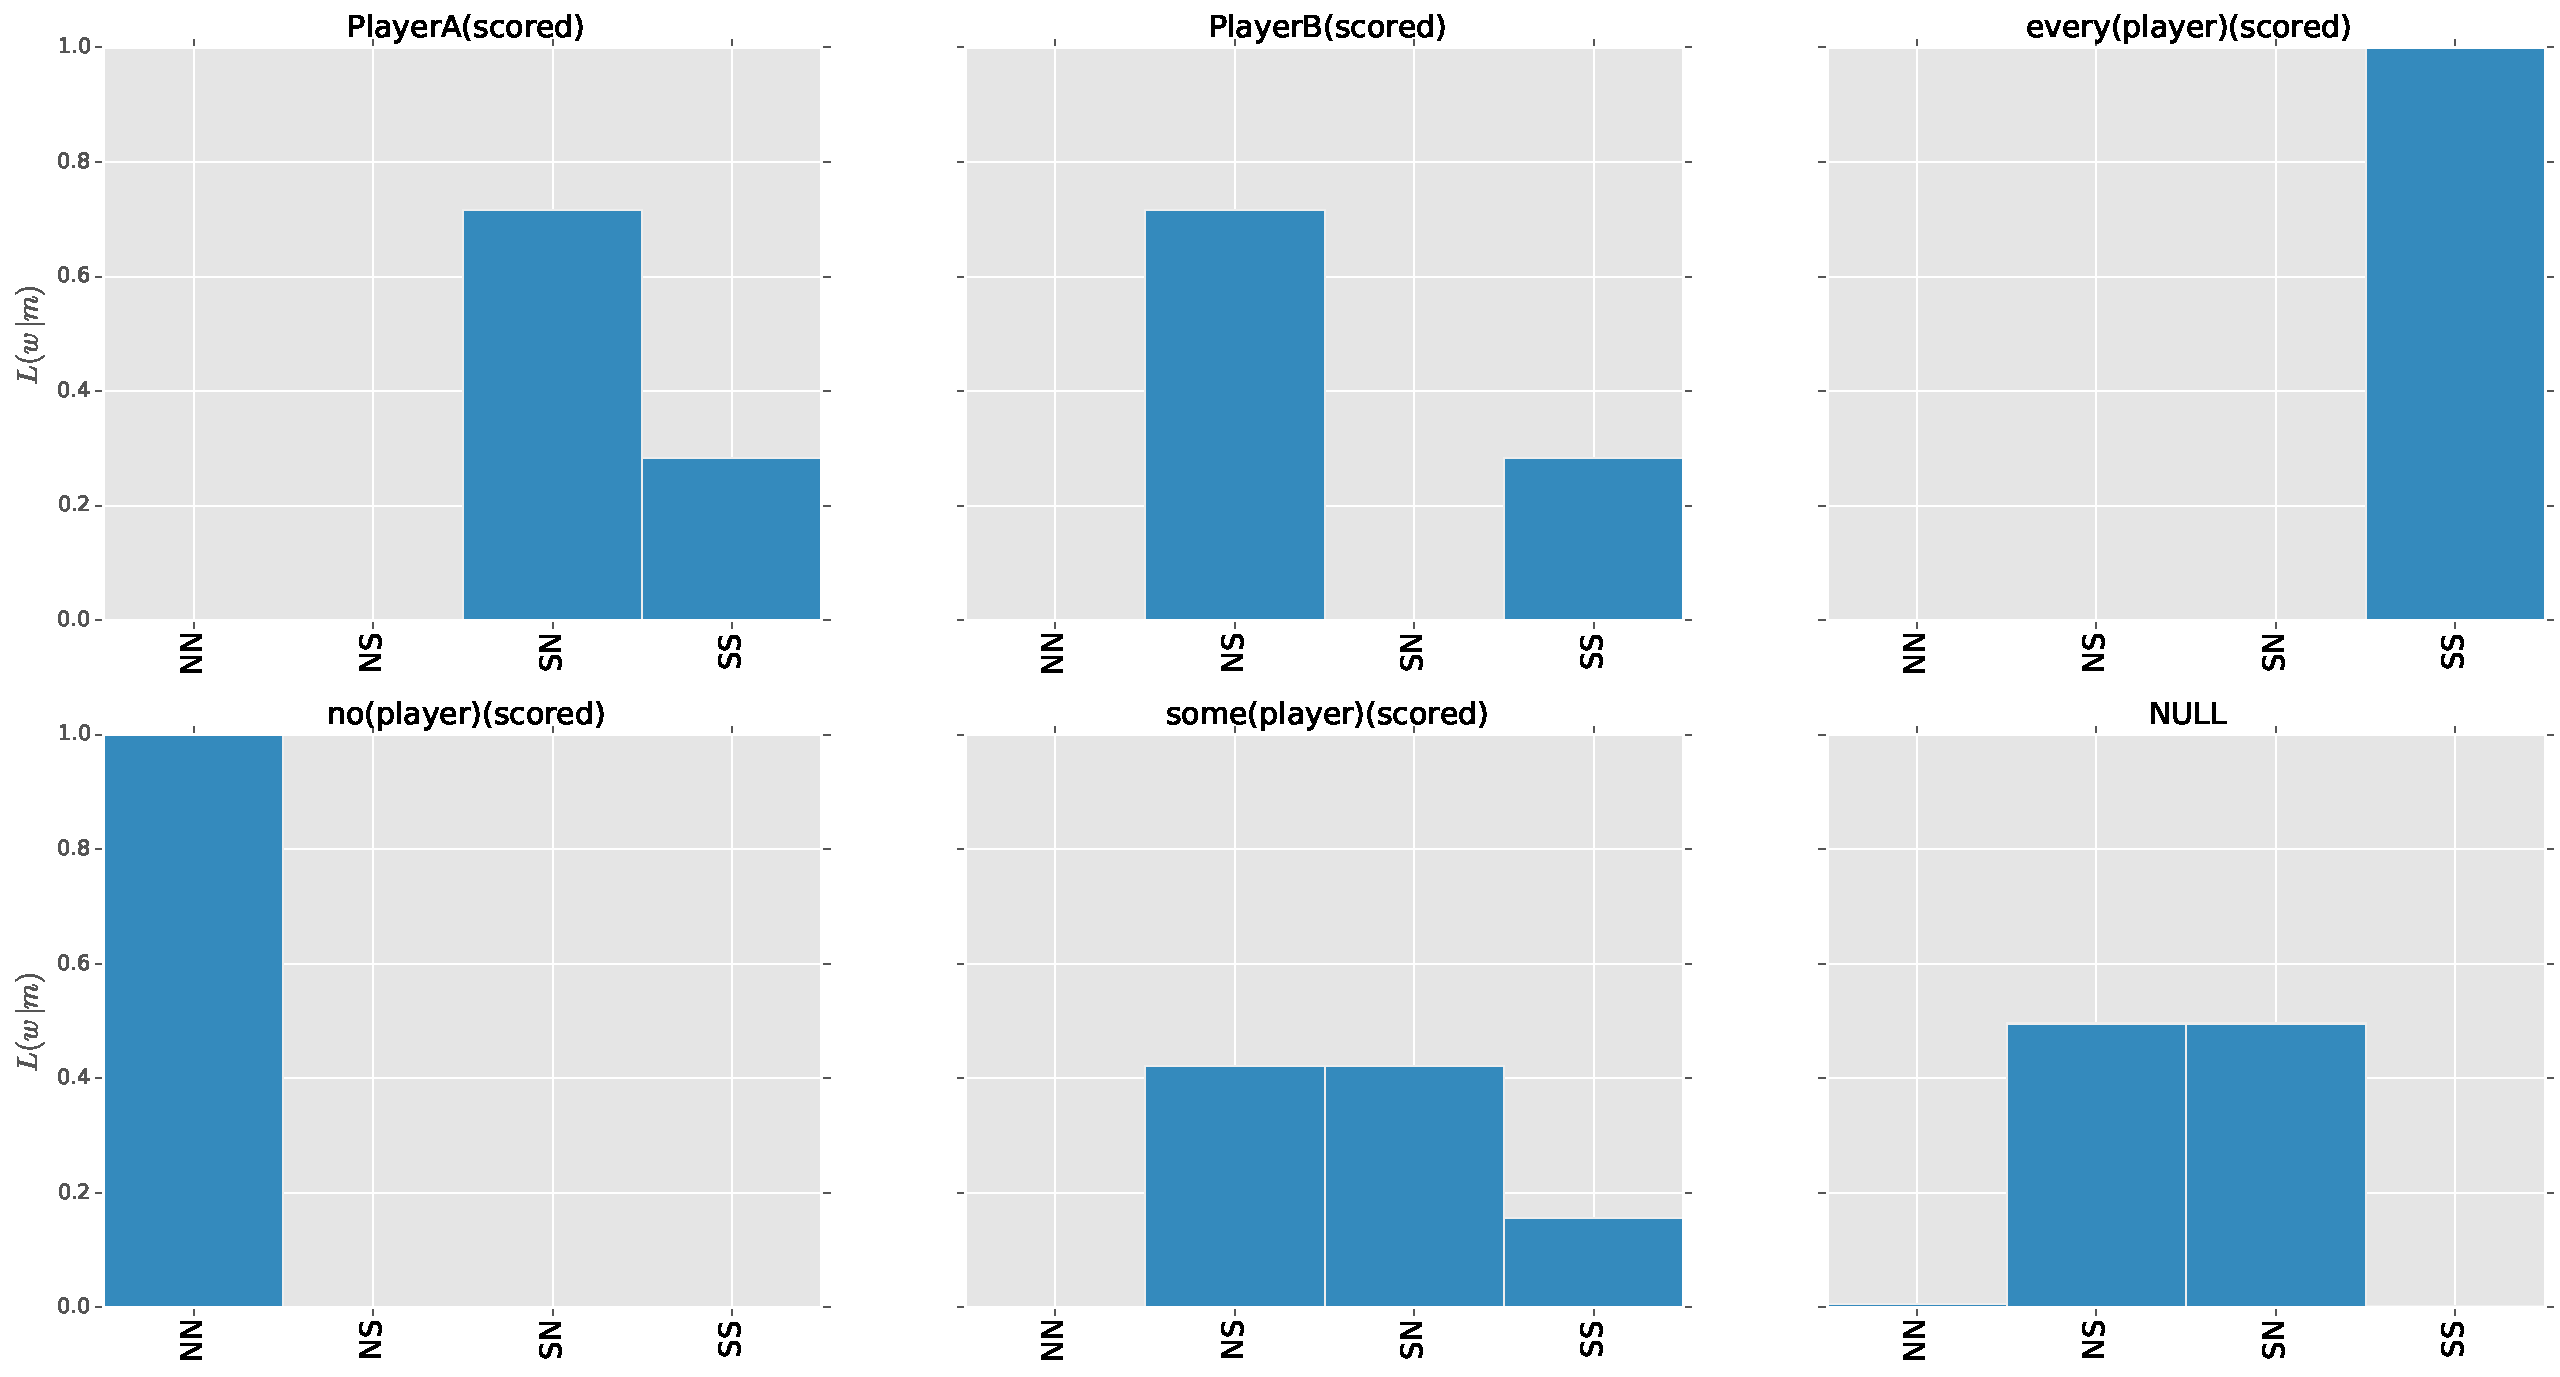
\includegraphics[width=0.8\textwidth]{fig/example-simple}
\end{examples}

%=====================================================================

%\newpage

\subsection{Subject refinement with added predicate refinement}

\begin{examples}
\item As above except we also allow the predicate \word{scored} to be
  refined as well.

\item

  \setlength{\tabcolsep}{8pt}
  \begin{tabular}[c]{r *{4}{r} }
    \toprule
    & NN & NS & SN & SS\\
    \midrule
    PlayerA(scored) & 0.0 & 0.0 & \graycell{0.58} & 0.42\\
    PlayerB(scored) & 0.0 & \graycell{0.58} & 0.0 & 0.42\\
    every(player)(scored) & 0.0 & 0.0 & 0.0 & \graycell{1.0}\\
    no(player)(scored) & \graycell{0.59} & 0.2 & 0.2 & 0.0\\
    some(player)(scored) & 0.0 & \graycell{0.38} & \graycell{0.38} & 0.23\\
    NULL & 0.02 & \graycell{0.49} & \graycell{0.49} & 0.0\\
    \bottomrule
  \end{tabular}

\item The overall picture is the same except the results for \word{no}
  are unintuitive. Here's why: if $\sem{\text{scored}}$ can be refined
  to just $\set{\playera}$, then \texttt{no(player)(scored)} comes out
  true in world \texttt{SN}. And similarly for refinement to just
  player $\set{\playerb}$. This results in a more even distribution
  than we would like (compare the comparable line in the previous
  example).
\end{examples}

%=====================================================================

\subsection{Predicate scalar implicatures}

\begin{examples}
\item

 \begin{examples}
  \item $\Worlds = \set{\texttt{NN}, \texttt{NS}, \texttt{NA}, \texttt{SN}, \texttt{SS}, \texttt{SA}, \texttt{AN}, \texttt{AS}, \texttt{AA}}$        
  \item $\Refinable = \set{\text{scored}, \text{doubled}}$
  \item $\Messages = \set{Q(P) : Q \in \set{\text{PlayerA}, \text{PlayerB}}, P \in \set{\text{scored}, \text{doubled}}}$
  \item $\lambda = 1$
  \item $\Costs(\nullmsg) = 5$; $\Costs(\msg) = 0$ for all $\msg \in \Messages-\set{\nullmsg}$  
  \item Flat state prior
  \item Flat lexicon prior
  \end{examples}

\item The predicate \word{doubled} is stronger than (entails)
  \word{scored}.

\item Our expectation is that \word{scored} will be enriched to
  exclude \word{doubled} --- a standard scalar implicture.

\item This results in 194,481 viable lexica. Of course, we can obtain
  this result without lexical uncertainty, but it's still nice to see
  that the result holds even after we churn through all those lexica:

  $\mspace{-120mu}$
  \setlength{\tabcolsep}{8pt}
  \begin{tabular}[c]{r *{9}{r} }
    \toprule
    & NN & NS & NA & SN & SS & SA & AN & AS & AA\\
    \midrule
    PlayerA(scored) & 0.0 & 0.0 & 0.0 & \graycell{0.27} & 0.2 & 0.13 & 0.17 & 0.13 & 0.1\\
    PlayerB(scored) & 0.0 & \graycell{0.27} & 0.17 & 0.0 & 0.2 & 0.13 & 0.0 & 0.13 & 0.1\\
    PlayerA(doubled) & 0.0 & 0.0 & 0.0 & 0.0 & 0.0 & 0.0 & \graycell{0.4} & 0.34 & 0.26\\
    PlayerB(doubled) & 0.0 & 0.0 & \graycell{0.4} & 0.0 & 0.0 & 0.34 & 0.0 & 0.0 & 0.26\\
    NULL & \graycell{0.34} & 0.17 & 0.07 & 0.17 & 0.08 & 0.04 & 0.07 & 0.04 & 0.02\\
    \bottomrule
  \end{tabular}
  
\end{examples}


%%%%%%%%%%%%%%%%%%%%%%%%%%%%%%%%%%%%%%%%%%%%%%%%%%%%%%%%%%%%%%%%%%%%%%
\newpage

\section{Experiment analysis}

\begin{examples}
\item

 \begin{examples}
  \item $\Worlds = \set{\texttt{NNN}, \texttt{NNS}, \texttt{NNA}, \texttt{NSS}, \texttt{NSA}, \texttt{NAA}, \texttt{SSS}, \texttt{SSA}, \texttt{SAA}, \texttt{AAA}}$    
  \item $\Refinable = \set{\text{some player}, \text{some shot}}$
  \item $\Messages = \set{Q(\text{player})(\text{made}(S(\text{shot}))) : Q \in \set{\text{exactlyone}, \text{every}, \text{no}}, S \in  \set{\text{every}, \text{no}, \text{some}}}$
  \item $\lambda = 1$
  \item $\Costs(\nullmsg) = 5$; $\Costs(\msg) = 0$ for all $\msg \in \Messages-\set{\nullmsg}$  
  \item $\StatePrior(w) = \StatePrior(w')$ for all $w, w' \in \Worlds$
  \item $\LexPrior(\Lex) = \LexPrior(\Lex')$ for all $\Lex, \Lex' \in \LexSet$
  \end{examples}

\item Goals given our experimental findings:
  \begin{examples}
  \item \texttt{every(player)(made(some(shot)))} should strongly favor \texttt{SSS}
  \item \texttt{exactlyone(player)(made(some(shot)))} should weakly favor \texttt{NNS}, but \texttt{SAA} and \texttt{NSA} should be contenders.
    (\texttt{NNA} is the unenriched case.)
  \end{examples}


\item Results with the listener's best inferences based on each state
  highlighted:

  $\mspace{-120mu}$
  \setlength{\tabcolsep}{4pt}
  \begin{tabular}[c]{r *{10}{r} }
    \toprule
    & NNN & NNS & NNA & NSS & NSA & NAA & SSS & SSA & SAA & AAA\\
    \midrule
    every(player)(made(every(shot))) & 0.0 & 0.0 & 0.0 & 0.0 & 0.0 & 0.0 & 0.0 & 0.0 & 0.0 & \graycell{1.0}\\
    every(player)(made(no(shot))) & \graycell{1.0} & 0.0 & 0.0 & 0.0 & 0.0 & 0.0 & 0.0 & 0.0 & 0.0 & 0.0\\
    every(player)(made(some(shot))) & 0.0 & 0.0 & 0.0 & 0.0 & 0.0 & 0.0 & \graycell{0.41} & 0.12 & 0.21 & 0.25\\
    exactlyone(player)(made(every(shot))) & 0.0 & 0.0 & \graycell{0.37} & 0.0 & 0.29 & 0.0 & 0.0 & 0.34 & 0.0 & 0.0\\
    exactlyone(player)(made(no(shot))) & 0.0 & 0.0 & 0.0 & 0.29 & 0.22 & \graycell{0.49} & 0.0 & 0.0 & 0.0 & 0.0\\
    exactlyone(player)(made(some(shot))) & 0.0 & \graycell{0.31} & 0.28 & 0.0 & 0.17 & 0.0 & 0.0 & 0.09 & 0.15 & 0.0\\
    no(player)(made(every(shot))) & 0.12 & \graycell{0.34} & 0.0 & 0.31 & 0.0 & 0.0 & 0.23 & 0.0 & 0.0 & 0.0\\
    no(player)(made(no(shot))) & 0.0 & 0.0 & 0.0 & 0.0 & 0.0 & 0.0 & 0.2 & 0.24 & \graycell{0.46} & 0.11\\
    no(player)(made(some(shot))) & \graycell{0.27} & 0.17 & 0.15 & 0.1 & 0.0 & 0.15 & 0.11 & 0.0 & 0.0 & 0.06\\
    NULL & 0.04 & 0.11 & 0.1 & 0.11 & 0.08 & \graycell{0.18} & 0.08 & 0.09 & \graycell{0.18} & 0.04\\
    \bottomrule
  \end{tabular}

\item Result also holds if \word{some} is allowed in the subject.

\item If \word{exactly one} is allowed in the object, then we still
  see the \word{every}/\word{some} result, but we lose the
  \word{exactly one}/\word{some} implicature. I think that's very
  intuitive --- if the speaker avoided salient and (in the above)
  equally costly \word{exactly one}, then she surely didn't intend its
  meaning.
  
\newpage

\item Plot of the above with the experimental results:

  $\mspace{-120mu}$
  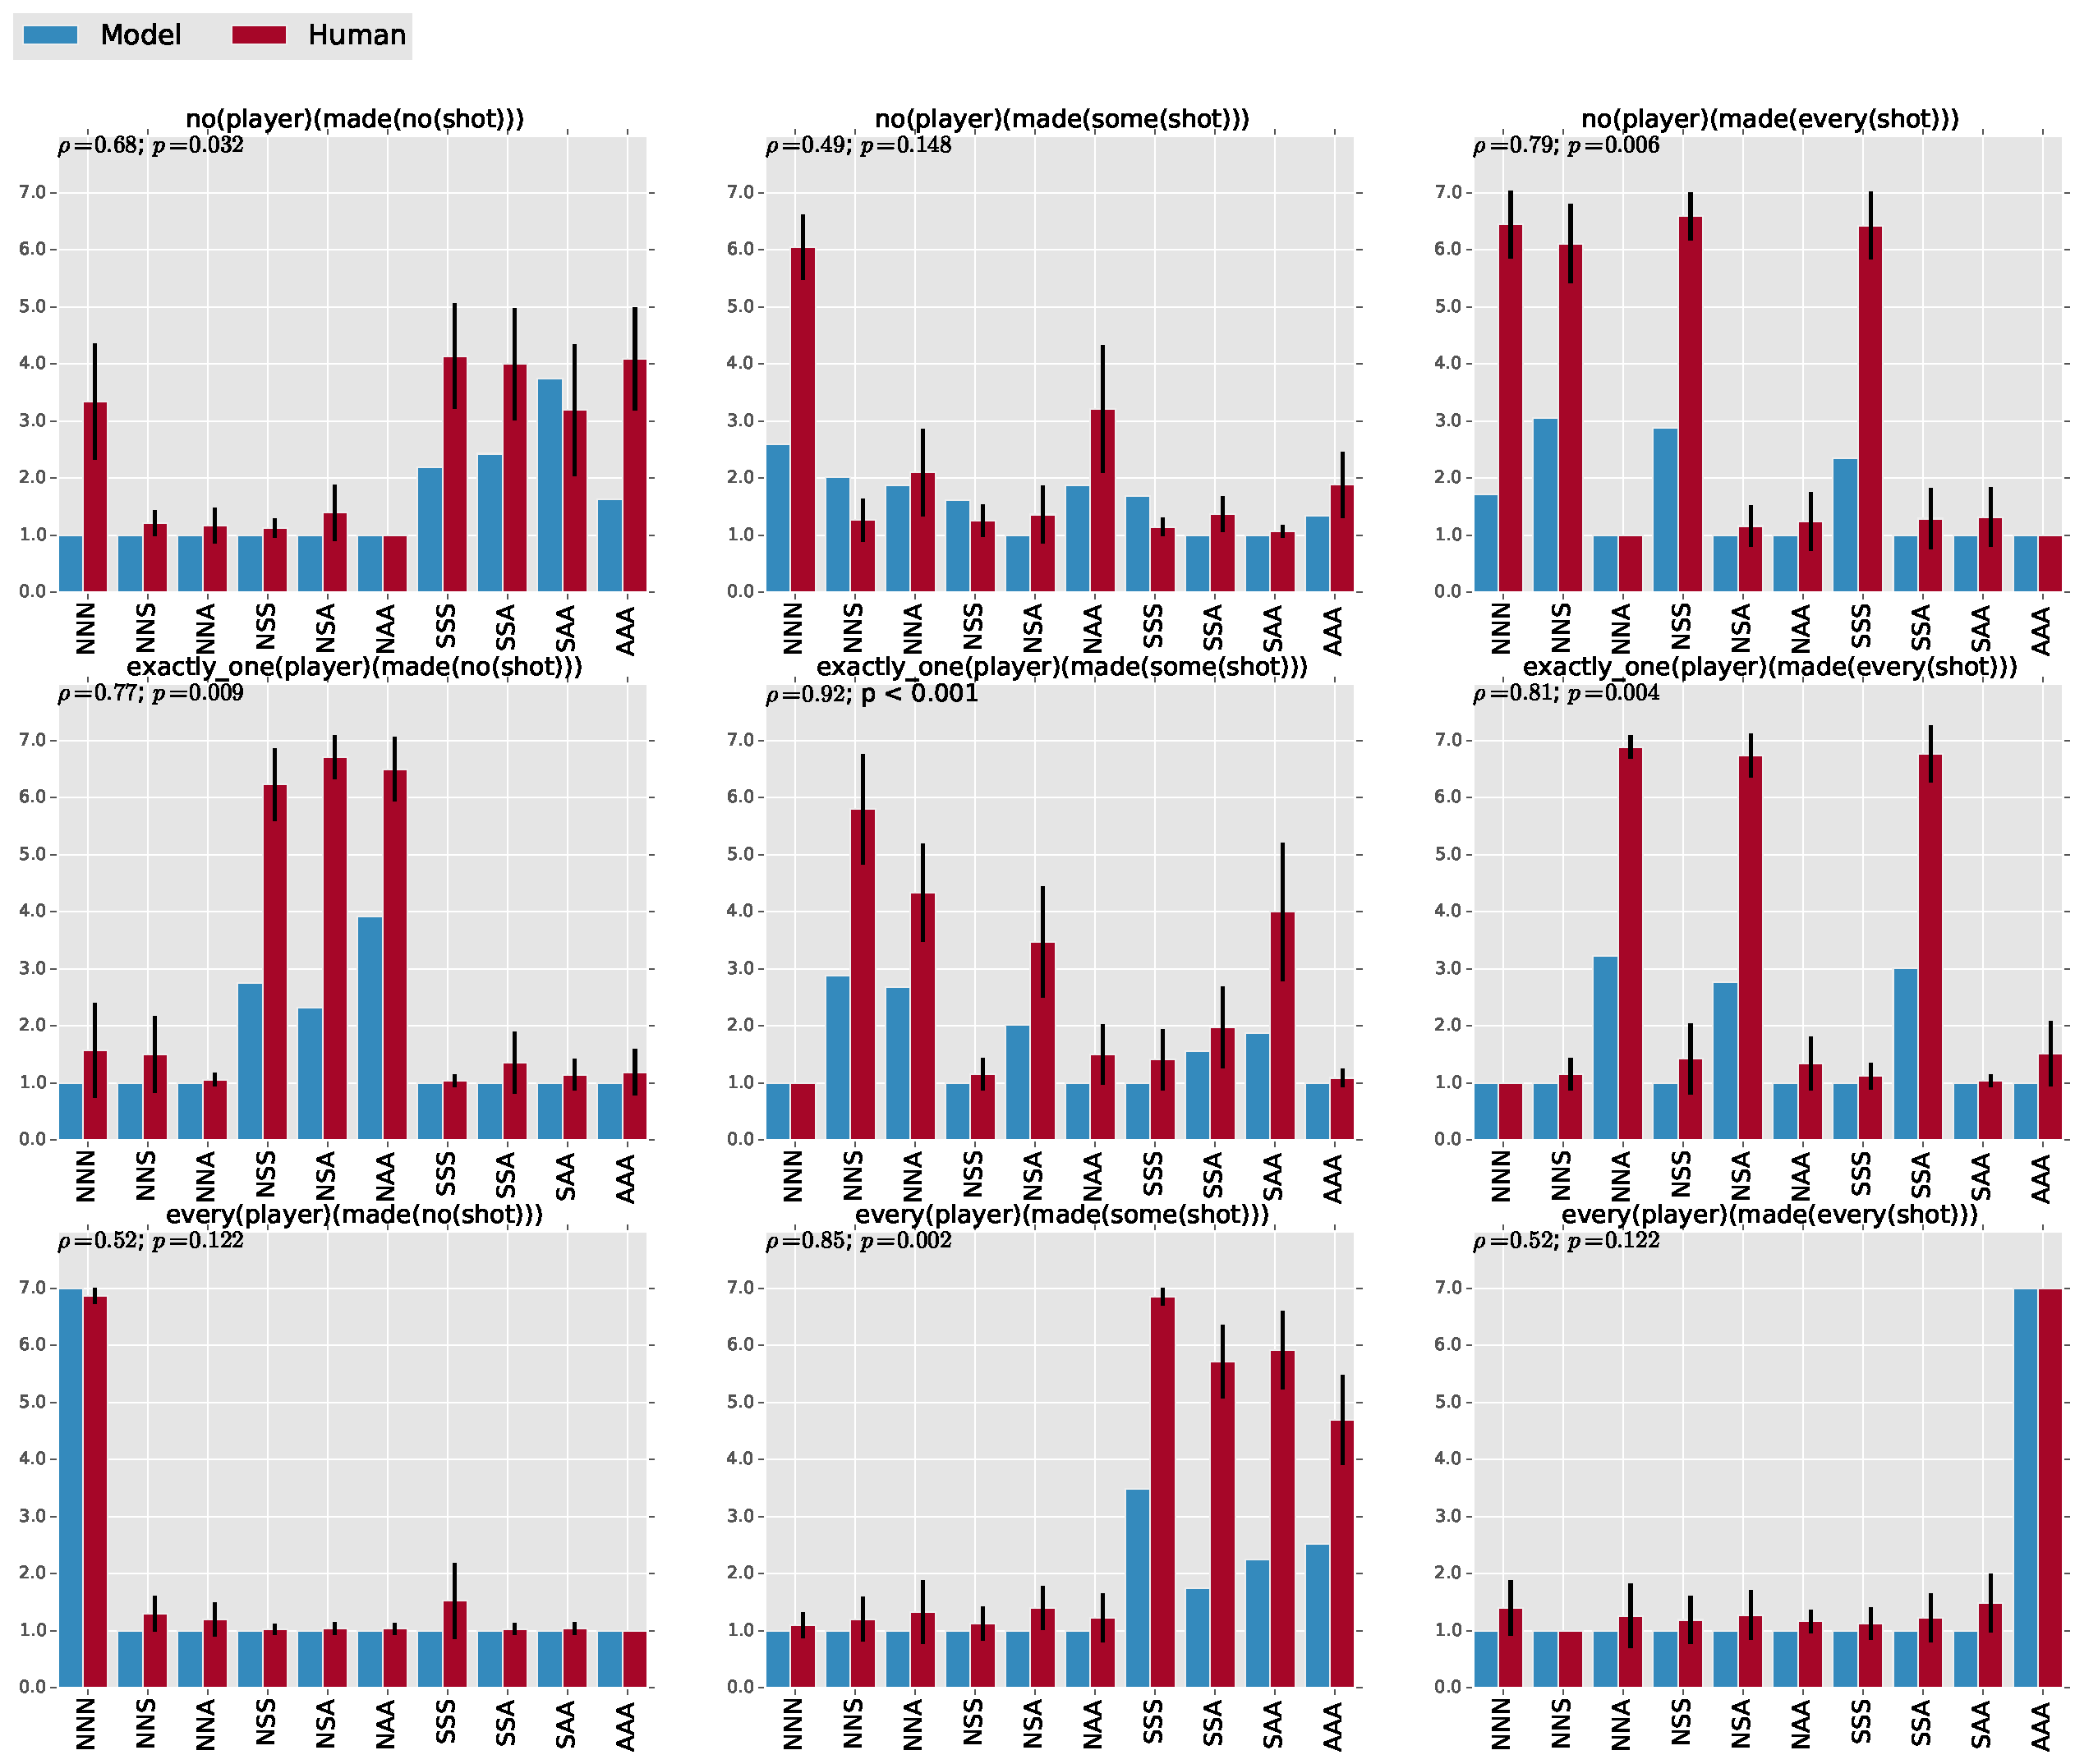
\includegraphics[width=1.2\textwidth]{fig/experiment-barplots}


\newpage

\item With the human judgments normalized as listener judgments:

  $\mspace{-120mu}$
  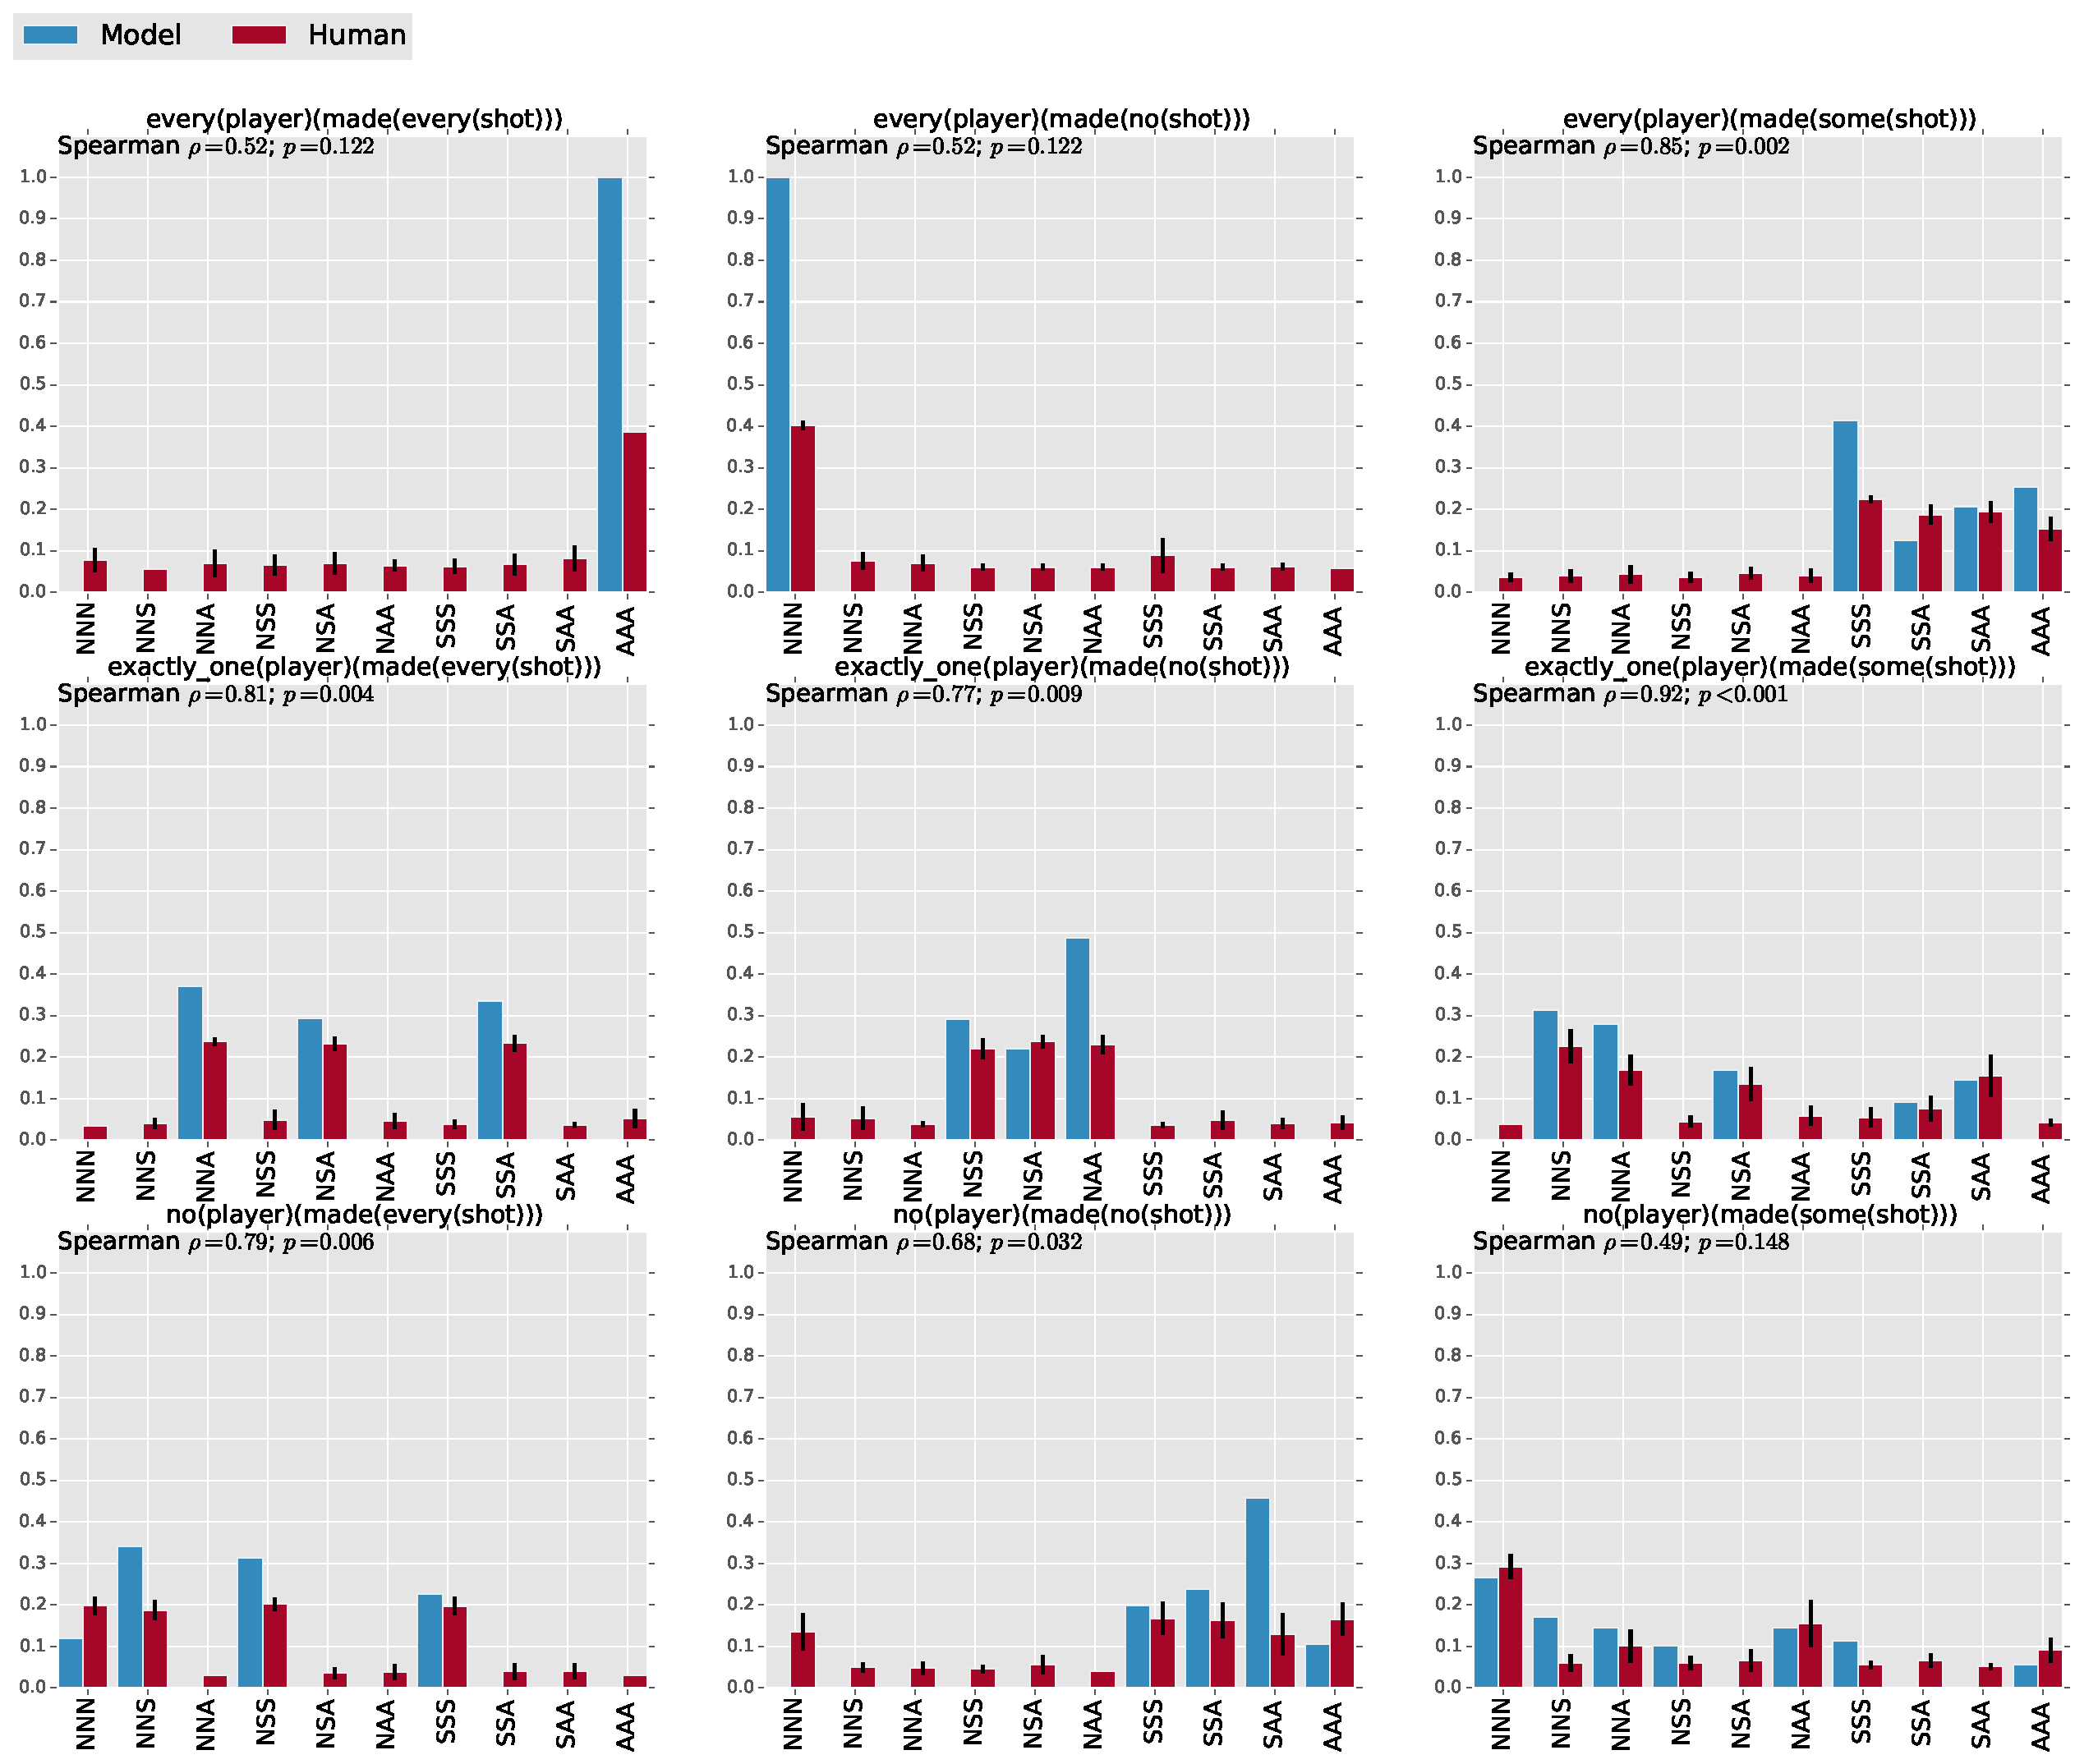
\includegraphics[width=1.2\textwidth]{fig/experiment-barplots-listenernorm}

\newpage

\item With the human judgments normalized as speaker judgments:

  $\mspace{-120mu}$
  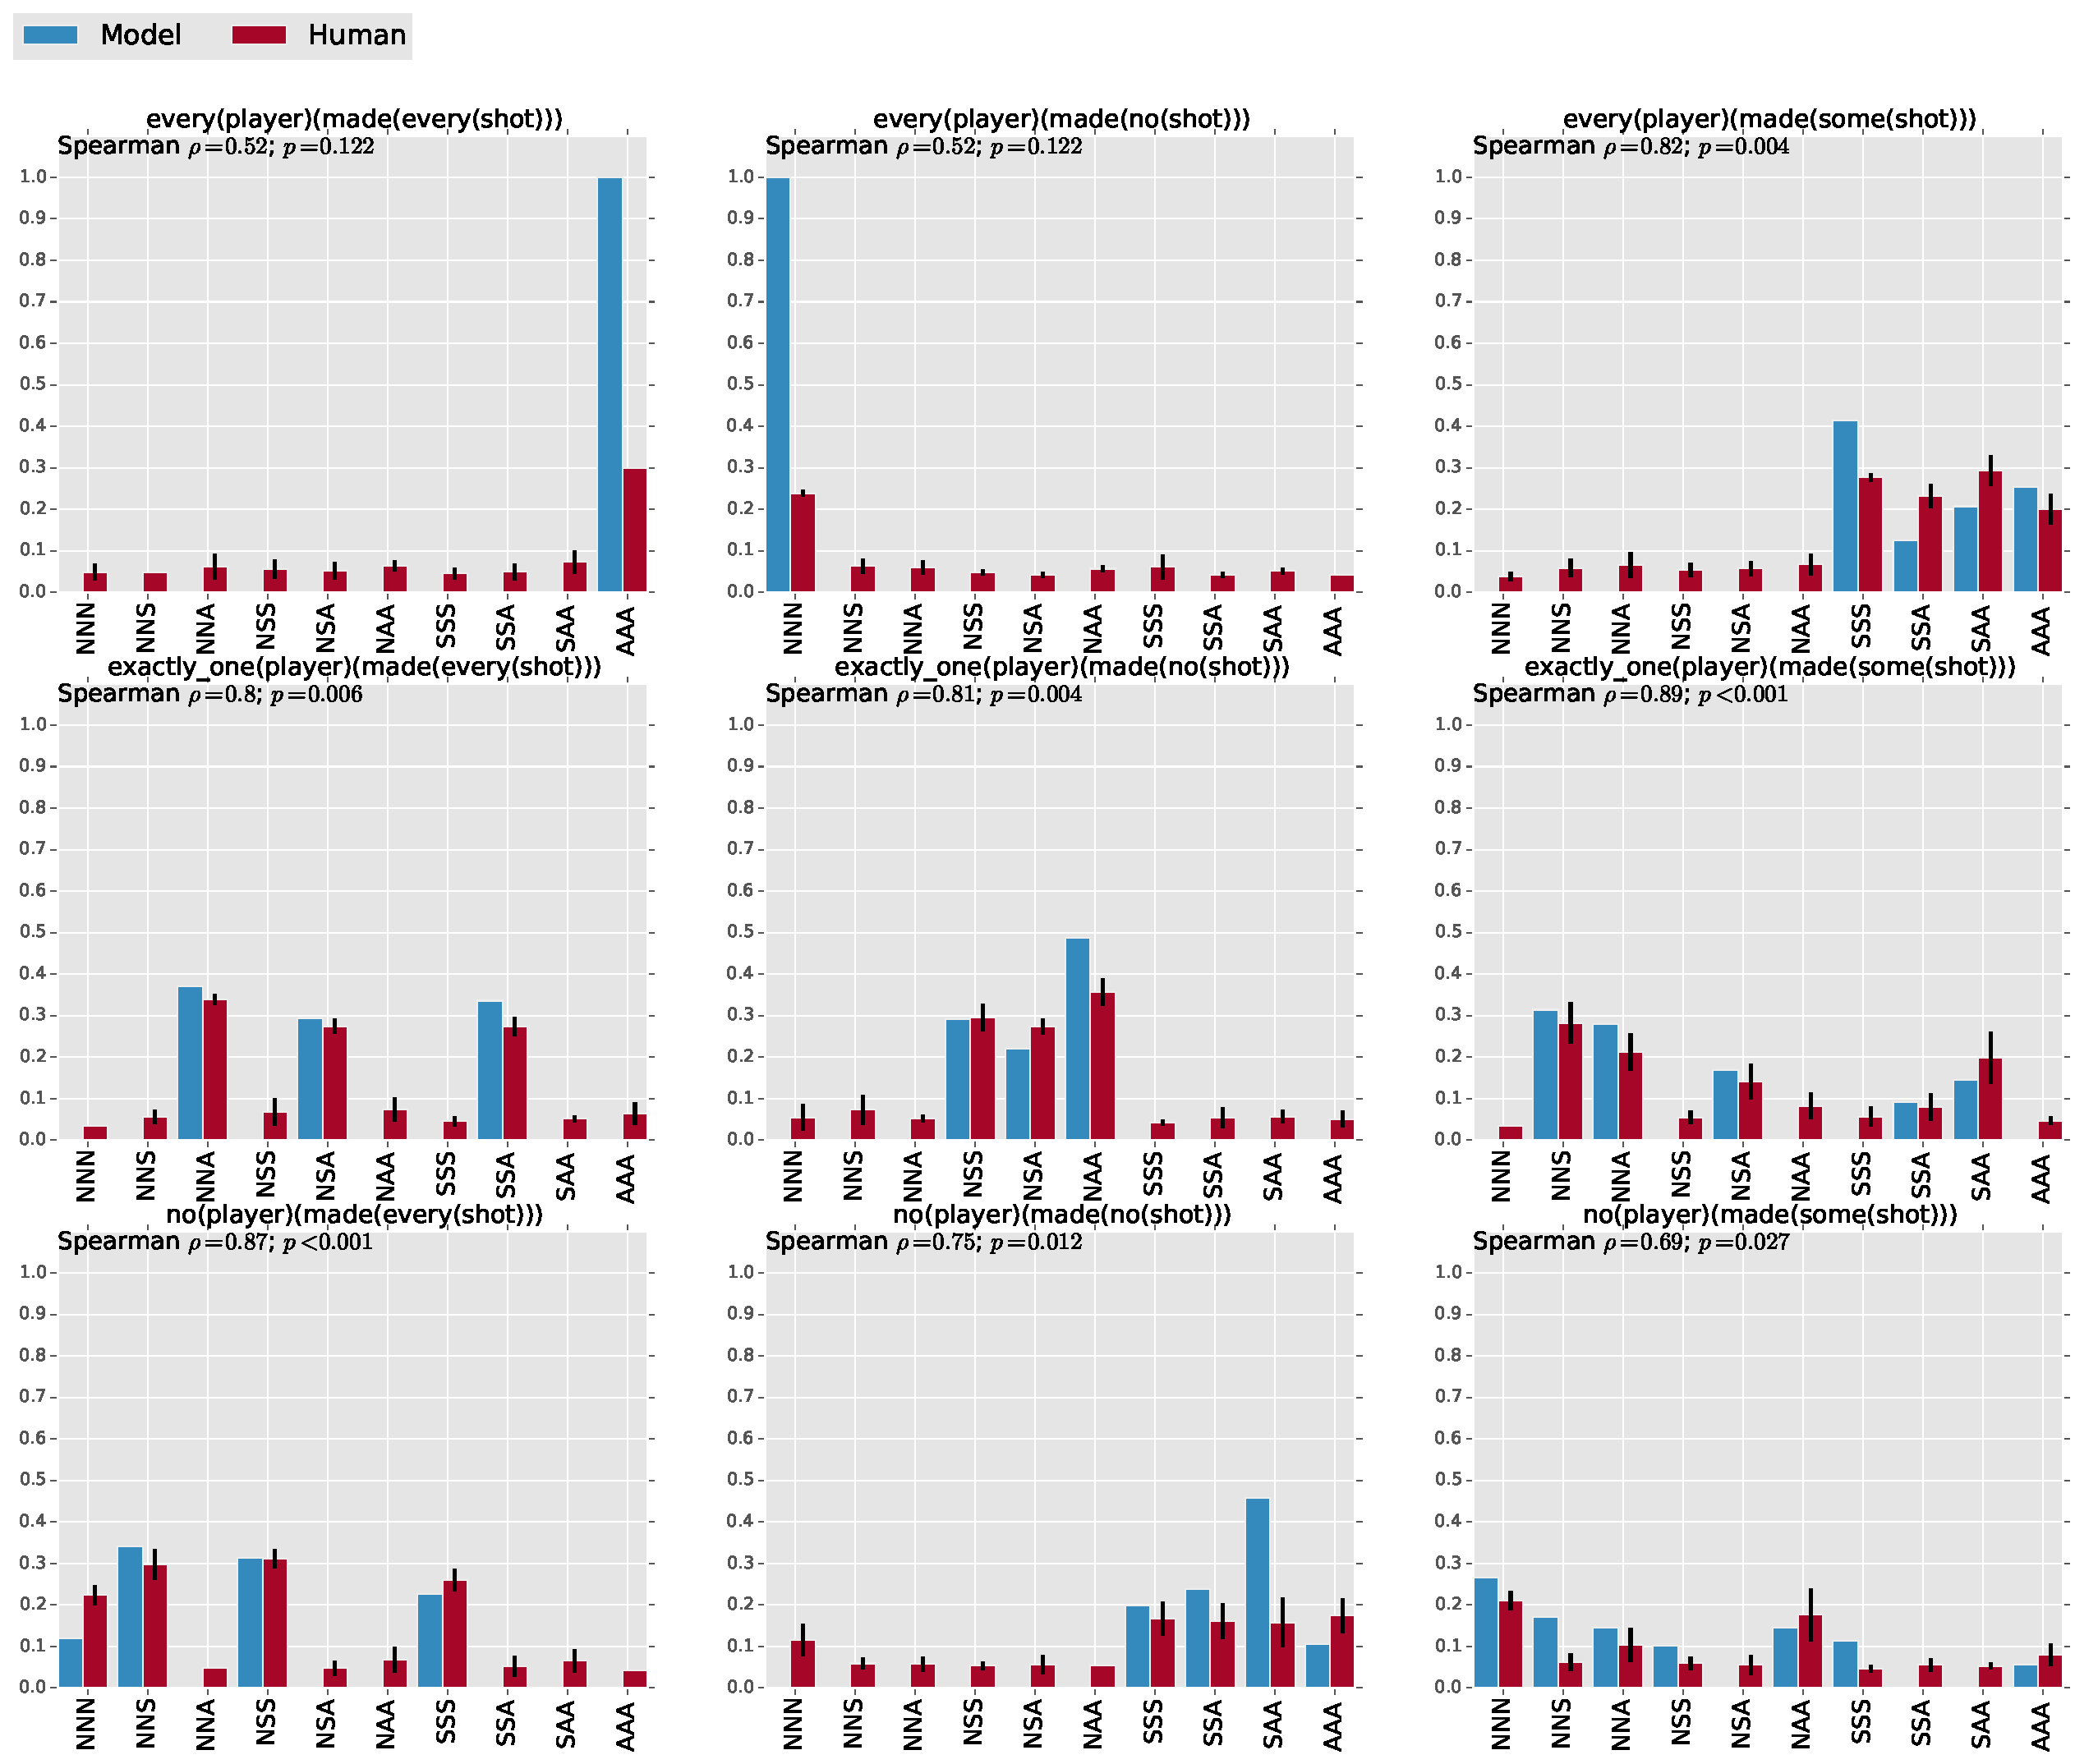
\includegraphics[width=1.2\textwidth]{fig/experiment-barplots-speakernorm}

\newpage

\item Correlation plot with the human data normalized as though it
  were a \textbf{listener} distribution (a simple rescaling of the
  raw data):

  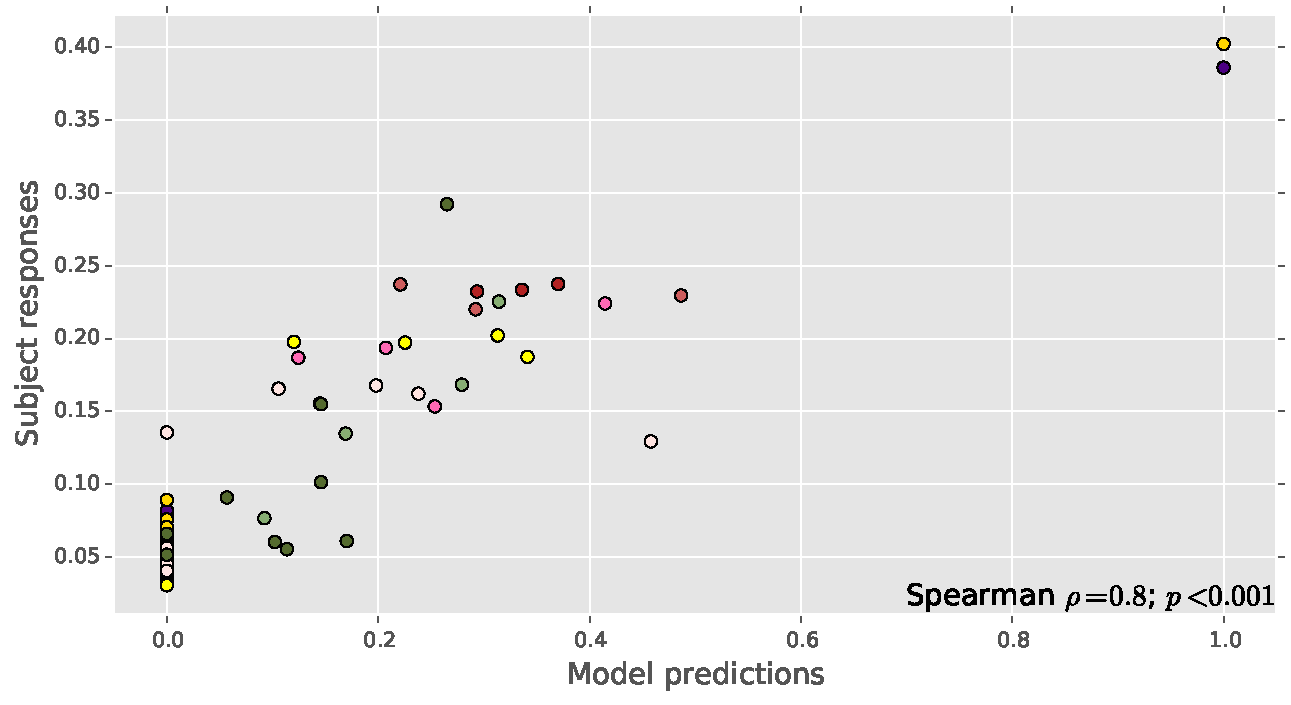
\includegraphics[width=1\textwidth]{fig/experiment-scatterplot-listenernorm.pdf}


\item Correlation plot with the human data normalized as though it
  were a \textbf{speaker} distribution:

  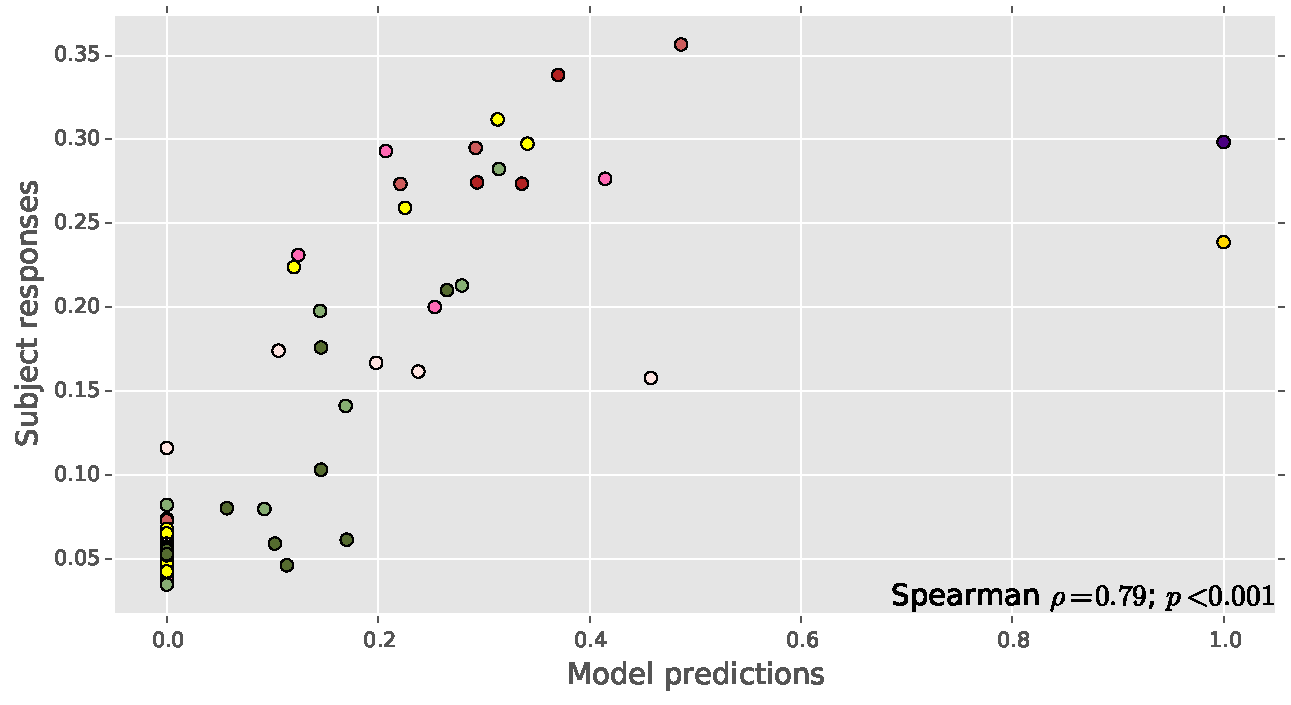
\includegraphics[width=1\textwidth]{fig/experiment-scatterplot-speakernorm.pdf}
\end{examples}

\newpage

%%%%%%%%%%%%%%%%%%%%%%%%%%%%%%%%%%%%%%%%%%%%%%%%%%%%%%%%%%%%%%%%%%%%%%

\section{Big example (just out of curiosity)}

\begin{examples}
\item

 \begin{examples}
  \item $\Worlds = \set{\texttt{NNN}, \texttt{NNS}, \texttt{NNA}, \texttt{NSS}, \texttt{NSA}, \texttt{NAA}, \texttt{SSS}, \texttt{SSA}, \texttt{SAA}, \texttt{AAA}}$    
  \item $\Refinable = \set{\text{some player}, \text{some shot}, \text{PlayerA}, \text{PlayerB}}$
  
    (No PlayerC because I was having issues holding the lexica in
    memory.)

  \item $\Messages = \set{A(\text{made}(B)) : A \in\textit{Subject}, B \in  \textit{Object}}$
    \begin{examples}
    \item $\textit{Subject} = \set{Q(\text{player}) : Q \in \set{\text{every}, \text{some}, \text{no}, \text{exactlyone}}} \cup \set{\text{PlayerA}, \text{PlayerB}, \text{PlayerC}}$
    \item $\textit{Object} = \set{Q(\text{shot}) : Q \in \set{\text{every}, \text{some}, \text{no}, \text{exactlyone}}}$
    \end{examples}
  \item $\lambda = 1$
  \item $\Costs(\nullmsg) = 5$; $\Costs(\msg) = 0$ for all $\msg \in \Messages-\set{\nullmsg}$  
  \item $\StatePrior(w) = \StatePrior(w')$ for all $w, w' \in \Worlds$
  \item $\LexPrior(\Lex) = \LexPrior(\Lex')$ for all $\Lex, \Lex' \in \LexSet$
  \end{examples}

\item Results with the listener's best inferences based on each state
  highlighted: 

  $\mspace{-120mu}$ 
  \setlength{\tabcolsep}{4pt}
  \renewcommand{\arraystretch}{0.9}
  \begin{tabular}[c]{r *{10}{r} }
    \toprule
    & NNN & NNS & NNA & NSS & NSA & NAA & SSS & SSA & SAA & AAA\\
    \midrule
    PlayerA(made(every(shot))) & 0.0 & 0.0 & 0.0 & 0.0 & 0.0 & 0.0 & 0.0 & 0.0 & 0.0 & \graycell{1.0}\\
    PlayerA(made(exactlyone(shot))) & 0.0 & 0.0 & 0.0 & 0.0 & 0.0 & 0.0 & \graycell{0.45} & 0.27 & 0.27 & 0.0\\
    PlayerA(made(no(shot))) & \graycell{0.27} & 0.15 & 0.17 & 0.14 & 0.12 & 0.16 & 0.0 & 0.0 & 0.0 & 0.0\\
    PlayerA(made(some(shot))) & 0.0 & 0.0 & 0.0 & 0.0 & 0.0 & 0.0 & 0.22 & 0.25 & 0.24 & \graycell{0.28}\\[1ex]
    PlayerB(made(every(shot))) & 0.0 & 0.0 & 0.0 & 0.0 & 0.0 & \graycell{0.37} & 0.0 & 0.0 & 0.3 & 0.33\\
    PlayerB(made(exactlyone(shot))) & 0.0 & 0.0 & 0.0 & \graycell{0.29} & 0.19 & 0.0 & 0.25 & 0.27 & 0.0 & 0.0\\
    PlayerB(made(no(shot))) & \graycell{0.36} & 0.3 & 0.34 & 0.0 & 0.0 & 0.0 & 0.0 & 0.0 & 0.0 & 0.0\\
    PlayerB(made(some(shot))) & 0.0 & 0.0 & 0.0 & 0.15 & 0.12 & \graycell{0.17} & 0.11 & \graycell{0.17} & \graycell{0.17} & 0.11\\[1ex]
    PlayerC(made(every(shot))) & 0.0 & 0.0 & 0.19 & 0.0 & 0.16 & \graycell{0.22} & 0.0 & 0.18 & 0.17 & 0.08\\
    PlayerC(made(exactlyone(shot))) & 0.0 & 0.38 & 0.0 & \graycell{0.42} & 0.0 & 0.0 & 0.2 & 0.0 & 0.0 & 0.0\\
    PlayerC(made(no(shot))) & \graycell{1.0} & 0.0 & 0.0 & 0.0 & 0.0 & 0.0 & 0.0 & 0.0 & 0.0 & 0.0\\
    PlayerC(made(some(shot))) & 0.0 & 0.15 & 0.11 & \graycell{0.18} & 0.1 & 0.13 & 0.07 & 0.11 & 0.11 & 0.04\\[1ex]
    every(player)(made(every(shot))) & 0.0 & 0.0 & 0.0 & 0.0 & 0.0 & 0.0 & 0.0 & 0.0 & 0.0 & \graycell{1.0}\\
    every(player)(made(exactlyone(shot))) & 0.0 & 0.0 & 0.0 & 0.0 & 0.0 & 0.0 & \graycell{1.0} & 0.0 & 0.0 & 0.0\\
    every(player)(made(no(shot))) & \graycell{1.0} & 0.0 & 0.0 & 0.0 & 0.0 & 0.0 & 0.0 & 0.0 & 0.0 & 0.0\\
    every(player)(made(some(shot))) & 0.0 & 0.0 & 0.0 & 0.0 & 0.0 & 0.0 & \graycell{0.37} & 0.16 & 0.16 & 0.32\\[1ex]
    exactlyone(player)(made(every(shot))) & 0.0 & 0.0 & \graycell{0.37} & 0.0 & 0.3 & 0.0 & 0.0 & 0.34 & 0.0 & 0.0\\
    exactlyone(player)(made(exactlyone(shot))) & 0.0 & 0.34 & 0.0 & 0.0 & 0.31 & 0.0 & 0.0 & 0.0 & \graycell{0.35} & 0.0\\
    exactlyone(player)(made(no(shot))) & 0.0 & 0.0 & 0.0 & 0.34 & 0.27 & \graycell{0.39} & 0.0 & 0.0 & 0.0 & 0.0\\
    exactlyone(player)(made(some(shot))) & 0.0 & 0.26 & \graycell{0.3} & 0.0 & 0.2 & 0.0 & 0.0 & 0.12 & 0.12 & 0.0\\[1ex]
    no(player)(made(every(shot))) & 0.16 & 0.32 & 0.0 & \graycell{0.36} & 0.0 & 0.0 & 0.17 & 0.0 & 0.0 & 0.0\\
    no(player)(made(exactlyone(shot))) & 0.15 & 0.0 & 0.34 & 0.0 & 0.0 & \graycell{0.38} & 0.0 & 0.0 & 0.0 & 0.14\\
    no(player)(made(no(shot))) & 0.0 & 0.0 & 0.0 & 0.0 & 0.0 & 0.0 & 0.17 & \graycell{0.34} & 0.33 & 0.15\\
    no(player)(made(some(shot))) & \graycell{0.31} & 0.13 & 0.14 & 0.13 & 0.0 & 0.15 & 0.07 & 0.0 & 0.0 & 0.06\\[1ex]
    some(player)(made(every(shot))) & 0.0 & 0.0 & 0.16 & 0.0 & 0.14 & \graycell{0.22} & 0.0 & 0.15 & 0.18 & 0.14\\
    some(player)(made(exactlyone(shot))) & 0.0 & 0.18 & 0.0 & \graycell{0.2} & 0.14 & 0.0 & 0.13 & 0.18 & 0.18 & 0.0\\
    some(player)(made(no(shot))) & 0.15 & 0.18 & \graycell{0.2} & 0.16 & 0.13 & 0.18 & 0.0 & 0.0 & 0.0 & 0.0\\
    some(player)(made(some(shot))) & 0.0 & 0.1 & 0.1 & 0.11 & 0.13 & 0.12 & 0.06 & 0.16 & \graycell{0.17} & 0.06\\
    NULL & 0.06 & 0.11 & 0.13 & 0.13 & 0.1 & \graycell{0.14} & 0.06 & 0.11 & 0.11 & 0.05\\
    \bottomrule
  \end{tabular}
\end{examples}

$\mspace{-100mu}$
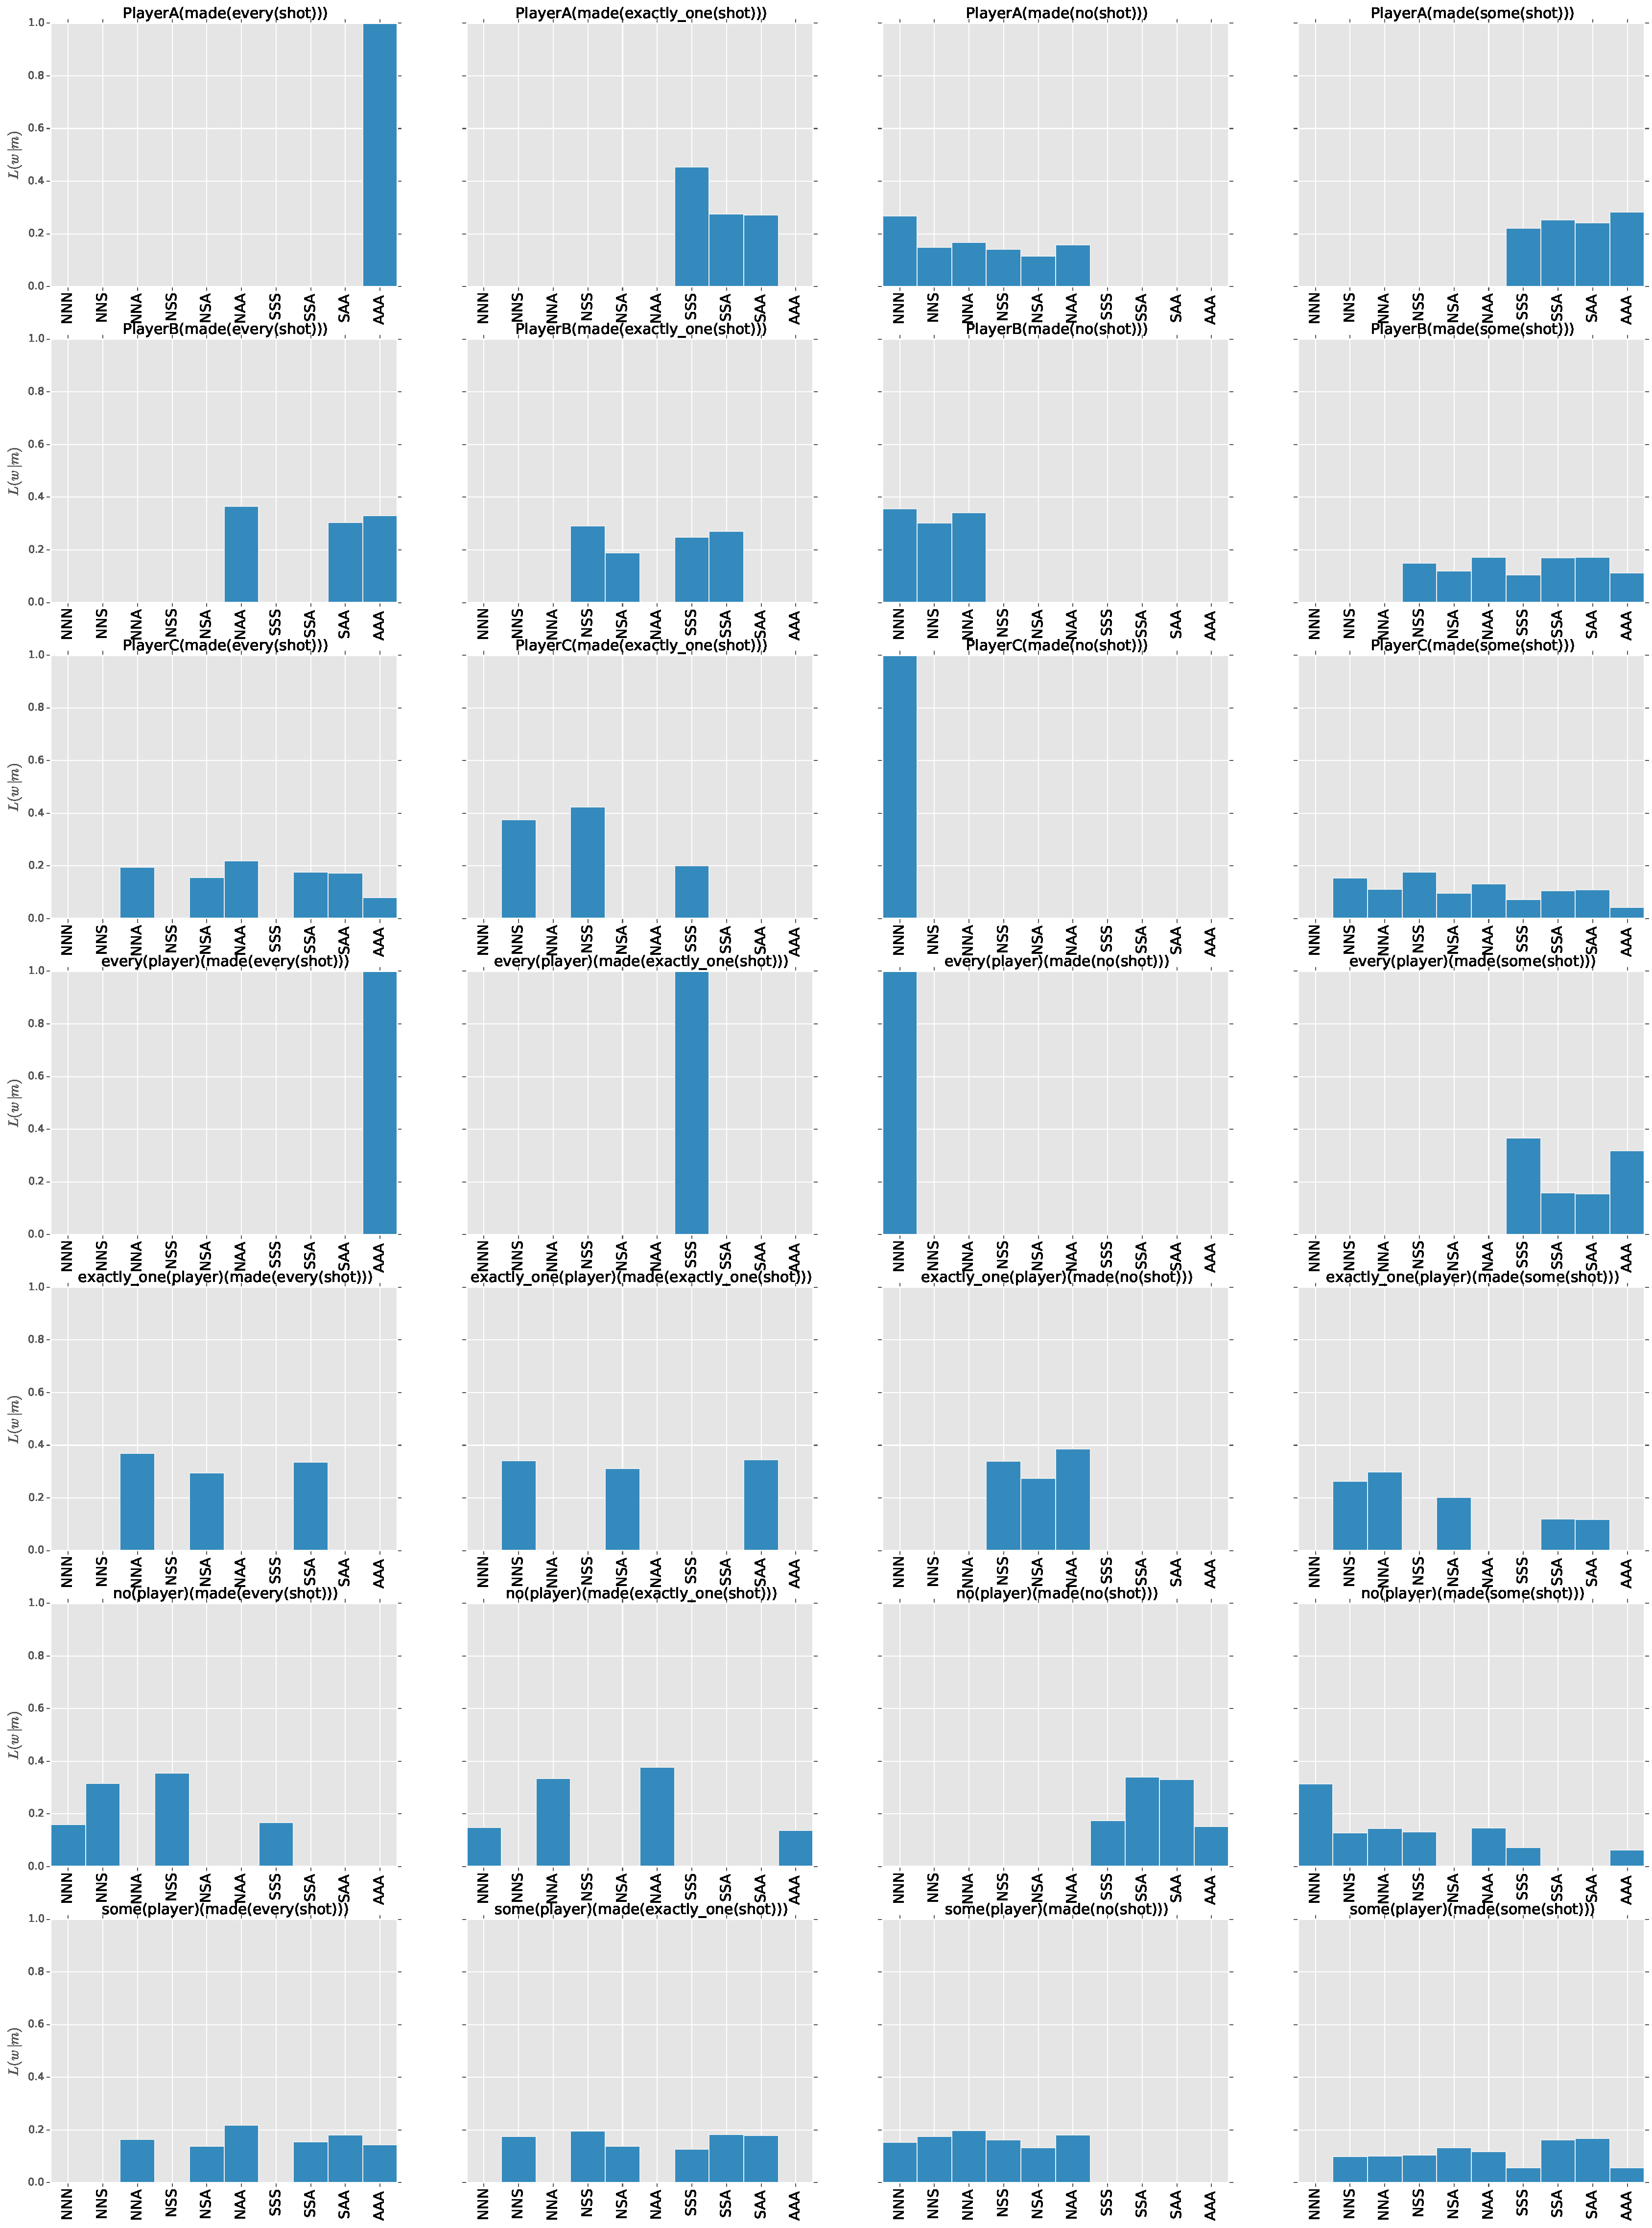
\includegraphics[width=1.2\textwidth]{fig/example-full}

%%%%%%%%%%%%%%%%%%%%%%%%%%%%%%%%%%%%%%%%%%%%%%%%%%%%%%%%%%%%%%%%%%%%%%

\section{Experimental evaluation of our model}\label{sec:experiments}

%=====================================================================

\subsection{Experiment 1: scalars under quantifiers}\label{sec:exp1}

\begin{examples}
\item Rationale: improve upon \citet{Chemla:Spector:2011} by using
  better items, more normal response patterns, and more standard
  assumptions about what the responses mean. Also perhaps make it
  easier to open things up to additional manipulations (e.g., QUDs).
\end{examples}

%=====================================================================

\subsection{Experiment 2: explicit exhaustification}\label{sec:exp2}

\begin{examples}
\item Rationale: \CFS\ use an operator that shares many
  characteristics with \word{only}. (This is part of the theoretical
  appeal, in that the operator seems to be needed anyway.)  Adding an
  explicit \word{only} gives us a sense for the pattern with explicit
  signaling --- a kind of upperbound on the effects we would expect.

\item Relevance for our model: adding \word{only} constrains the space
  of alternatives in ways that boost the strength of the embedding and
  basically/fully remove the need for pragmatic reasoning.  
\end{examples}

%=====================================================================

\subsection{Experiment 3: prosodic focus}\label{sec:exp3}

\begin{examples}
\item Rationale: \CFS's operator is also closely related to what one
  expects on accounts of topic and focus intonation that are based in
  alternatives. The \ALT\ operator embodies one of many things that
  one might do pragmatically with alternatives (negate them; in other
  contexts, they could be affirmed, highlighted because of speaker
  ignorance, etc.). Thus, we might expect prosodic focus to boost the
  signal.

\item Relevance for our model: harder to say. We could assume that
  focus alternatives are somehow part of the messages. We could also
  see what happens when focal forms are simply made more costly (in
  terms of the cost function $\Costs$) than their unfocussed
  counterparts.
\end{examples}

%%%%%%%%%%%%%%%%%%%%%%%%%%%%%%%%%%%%%%%%%%%%%%%%%%%%%%%%%%%%%%%%%%%%%%

\bibliographystyle{apalike}
\bibliography{embedded-scalars-bib}


\end{document}
